\documentclass[11pt, a4paper, oneside]{book}

\usepackage{fancyhdr}
\pagestyle{fancy}
\fancyhf{}

\usepackage[english]{babel}
\usepackage{graphicx}
\usepackage[colorlinks,hyperindex,plainpages=false,breaklinks]{hyperref}
\usepackage{amssymb}
\usepackage{wasysym} 
\usepackage{wrapfig}
\usepackage{enumerate}
\usepackage{placeins} % Necessary for \FloatBarrier
\usepackage{subfig}   % Necessary for subfloat (images next to each other)
\usepackage{color}
\usepackage[usenames,dvipsnames,svgnames]{xcolor}
\usepackage{listings}

\definecolor{codelightgray}{rgb}{0.87,0.87,0.87}

\hypersetup{colorlinks=true,% 
	linkcolor=black,%
	citecolor=red,%
	filecolor=blue,% 
	menucolor=black,% 
	pagecolor=black,%
	urlcolor=black
}

\lstset{language=,
    keywordstyle=\color{blue},
    basicstyle=\scriptsize\ttfamily,
    showstringspaces=false,
    backgroundcolor=\color{codelightgray},
    morekeywords={SELECT,FROM,WHERE,AND,OR,EClass}
}

% Set TOC Depth
\setcounter{tocdepth}{1}

\setlength{\parindent}{0pt} 
\setlength{\parskip}{0.3cm}

% Remove section numbers 0.1, 0.2 ..
\renewcommand{\thesection}{\arabic{section}} 

\graphicspath{%
{../../06_miscellaneous/commonFiles/}% Title image and memBox illustration
{../01_LeitnersBoxReviewed/lbrImages/}%
{../02_transformationsExplained/teImages/}%
{../03_removeCard/splashImages/}{../03_removeCard/GUIImages/}%
{../03_removeCard/visRemImages/}{../03_removeCard/texRemImages/}%
{../04_checkCard/splashImages/}{../04_checkCard/visCheImages/}{../04_checkCard/texCheImages/}%
{../05_emptyPartition/}{../05_emptyPartition/visEPImages/}{../05_emptyPartition/texEPImages/}%
{../06_invertCard/}{../06_invertCard/visICImages/}{../06_invertCard/texICImages/}%
{../07_growBox/}{../07_growBox/injectionsRevisited/irImages/}{../07_growBox/injections/iImages/}{../07_growBox/visGBImages/}{../07_growBox/texGBImages/}%
{../08_stringRep/}{../08_stringRep/injectionsReReVisited/irrImages/}{../08_stringRep/visSRImages/}{../08_stringRep/texSRImages/}%
{../09_fastCards/}{../09_fastCards/visFCImages/}{../09_fastCards/texFCImages/}%
{../10_conditionalBranching/}{../10_conditionalBranching/splashImages/}{../10_conditionalBranching/visCBImages/}{../10_conditionalBranching/texCBImages/}%
{../11_LLBGuiExtended/}%
}


% --- HEADER FUNCTIONS ----------------------------------------------------------------------------------------------------------------------------------------
% Default plain header; turn off all lines and colors; turn on page numbers for all
\newcommand{\noHeader}{
	\fancyfoot{}
 	\fancyhead[R]{\thepage}
	\fancyhead[L]{}
	\renewcommand{\headrulewidth}{0pt}
}

% Common instruction Header; Black
\newcommand{\genHeader}{
	\fancyfoot{}
	\fancyhead[L]{}
	\renewcommand{\headrulewidth}{1.5pt}
 	\renewcommand{\headrule}{\hbox to\headwidth{%
  		\color{Black}\leaders\hrule height \headrulewidth\hfill}}
}

% Visual instructions; Red header
\newcommand{\visHeader}{
	\fancyfoot{}
	\fancyhead[L]{\color{RedOrange}\tiny \bf VISUAL}
	\renewcommand{\headrulewidth}{1.5pt}
	\renewcommand{\headrule}{\hbox to\headwidth{%
  		\color{RedOrange}\leaders\hrule height \headrulewidth\hfill}}
}

% Text instructions; Blue header
\newcommand{\texHeader}{
	\fancyfoot{}
	\fancyhead[L]{\color{CornflowerBlue}\tiny \bf TEXTUAL}
	\renewcommand{\headrulewidth}{1.5pt}
	\renewcommand{\headrule}{\hbox to\headwidth{%
  		\color{CornflowerBlue}\leaders\hrule height \headrulewidth\hfill}}
}
% -------------------------------------------------------------------------------------------------------------------------------------------------------------


\newcommand{\requiredTime}[1]{ {\scriptsize \texttt{Approximate time to complete: #1} } }

% Jump links 
\newcommand{\jumpSingle}[1]{
\fancyfoot[OR]{$\triangleright$ \hyperlink{#1}{\texttt{Next}}}
}

\newcommand{\jumpDual}[2]{
\fancyfoot[RO]{ $\triangleright$ \hyperlink{#1}{\texttt{Next [visual]\hspace{0.2cm}}}%
 \\ $\triangleright$ \hyperlink{#2}{\texttt{Next [textual]}}}
}

% These words should appear in the glossary
\newcommand{\define}[1]{ \marginpar{\small\emph{#1}} }

% Text syntax/command format
\newcommand{\syntax}[1]{ \begin{quote} \small \texttt{#1} \end{quote}}	

% Quick author note; remove from final
\newcommand{\update}{{\bf update}}

% TODO: update description download link
\newcommand{\dlPartZero}{\url{http://www.emoflon.org/}}

% TODO:  Update version number (Title Page Information)--------------------------------------------------------------------------------------------------------
\def\partTitle{Part III: Story Driven Modelling}
\def\versionNumber{0.1}
\title{
\flushright
{\LARGE\bfseries An Introduction to Metamodelling\\
and Graph Transformations}
\noindent\rule[-1ex]{\textwidth}{5pt}\\[2.5ex]
\hfill\emph{\LARGE\bfseries with eMoflon}\\
\vspace{1cm}
\includegraphics[width=0.85\textwidth]{pics/eMoflon3} 
}

\date{}  
\author{} 
% -------------------------------------------------------------------------------------------------------------------------------------------------------------

\begin{document}

\frontmatter
\noHeader

% Title Page without trailing blank page
{\let\newpage\relax\maketitle}

% Copyright notice
\begin{small} 
Copyright \copyright~2011--\the\year{} Real-Time Systems Lab, TU Darmstadt.
Anthony Anjorin, Erika Burdon, Frederik Deckwerth, Roland Kluge, Marius Lauder,
Erhan Leblebici, Daniel T\"ogel, David Marx, Lars Patzina, Sven Patzina, Alexander Schleich, Sascha Edwin Zander, Jerome Reinl\"ander, Martin Wieber, and contributors.
All rights reserved.

This document is free; you can redistribute it and/or modify it under the terms of the GNU Free Documentation License as published by the Free Software Foundation; either version 1.3 of the License, or (at your option) any later version.
Please visit \href{http://www.gnu.org/copyleft/fdl.html}{http://www.gnu.org/copyleft/fdl.html} to find the full text of the license.
 
% TODO Remove this?? It can be found easily online .. (we can even offer it on
% the download page) For your convenience, this document includes a copy of the \emph{GNU General Public License} starting from page~\pageref{chap:gpl}.
  
For further information contact us at \eMoflonContact.
  
\vskip3cm
\textit{The eMoflon team}\\
Darmstadt, Germany (\monthword{\month} \the\year)
\end{small}
\let\cleardoublepage\clearpage

% TOC
\tableofcontents
	
% Store page counter
\newcounter{romanpages}
\setcounter{romanpages}{\value{page}}

\mainmatter

% Main content for this Part 
\vspace*{2cm}

{\bf \huge Part III:}
\vspace{1cm}

{\bf \Huge Story Driven Modeling }
\vspace{1cm}

\genHeader
\requiredTime{haven't decided yet}

Welcome to Part III, an introduction to unidirectional model transformations via programmed graph transformations using Story Driven Modeling (SDM).
SDMs focus on concrete implementations, so we plan to implement the methods signatures declared in the abstract styntax. It other words, this is where you'll
build your metamodel's dynamic semantics! Don't let the sheer size of this part frighten you off - we have included deep, thorough explanations with many
figures to ensure the concepts are crystal clear. It's really not that bad.

In Part II, we learned that we can implement methods in a straightforward manner with injections and Java code, so why bother with SDMs? 

Overall, SDMs are simply an alternate way of implementing methods. Rather than verbose Java code, you can model each task, then generate the implementation
code to incorporate the idea into existing code. With the visual syntax, the advantage is obvious. You'll be able to use familiar, easy-to-understamd UML
activity diagrams to establish your methods. Texually, SDMs extend the Objected Oriented Paradigm and separates all classes, references and links, and
activities into separate files, folders, and patterns.

% That was the advantage, but WHY do we use SDMs? (Motivation)

If you're just joining us, read the next section for a brief overview of our running example so far, and how to download some files that will help you get
started right away. If you're continuing from Part II, click the link below to continue with your constructed learning box metamodel.

\begin{center}\texttt{$\triangleright$ \hyperlink{explanation}{Continue from Part II\ldots}}\end{center}


\section{Leitner's learning box reviewed}

% Mention the visual validation tool?
\emph{Leitner's learning box}\footnote{\href{http://en.wikipedia.org/wiki/Leitner\_system}{http://en.wikipedia.org/wiki/Leitner\_system}} is a simple, but
ingenious little contraption to support the tedious process of memorization, especially prominent when trying to learn, for example, a new language. As depicted in
Fig.~\ref{fig:membox_depiction}, this box consists of a series of partitions with a strict set of rules. The contents to be memorized are written on little cards and placed in the first container. Every
time the user correctly answers a card, that card is promoted to the next partition. Once it reaches the final partition, it can be considered memorized, and
no longer needs to be practiced. Every time the user incorrectly answers a card however, it is sent back to the original starting partition, and the
learning process is restarted.

\begin{figure}[htbp]
	\centering
  \includegraphics[width=0.4\textwidth]{membox_illustration.pdf}
	\caption{Static Structure of a Leitner's Learning Box}
	\label{fig:membox_depiction}
\end{figure}

For a more detailed overview of the box and our goals, we recommend you read the introduction to Part II. But for now, enough discussion!

\begin{itemize}

\item[$\blacktriangleright$] To get started, press the \texttt{new} button and navigate to ``Examples/eMoflon Handbook Examples/''
(Fig.~\ref{fig:downloadWizard}).

\begin{figure}[htbp]
	\centering
  \includegraphics[width=0.75\textwidth]{eclipse_downloadWizard}
	\caption{Download the file set to get started}
	\label{fig:downloadWizard}
\end{figure}

\item[$\blacktriangleright$] Download the file package of the eMolfon syntax type you'd like to learn about. Remember, with the visual syntax, you'll be using
an external modeling program to craft your metamodel diagrams, then exporting the data to Eclipse. With textual, you'll be working entirely within the
Eclipse IDE in the eMolfon perspective.

\newpage

\vspace*{0.5cm}

\item[$\blacktriangleright$] If your package explorer does not resemble ours in Fig.~\ref{fig:workingSets} with at least two distinct nodes, select the
small, downward facing arrow in the corner of the module window. Choose ``Working Sets'' as your ``Top Level Elements''. We use these to structure the workspace
in Eclipse.

\vspace{0.75cm}

\end{itemize}

\begin{figure}[htbp]
	\centering
  \includegraphics[width=0.9\textwidth]{eclipse_workingSets}
	\caption{Setting your Package Explorer}
	\label{fig:workingSets}
\end{figure}

The ``MyWorkingSet" node contains \texttt{LeitnersLearningBox}, which in turn contains all the metamodel project files. Visually, this is represented in a
single \texttt{.eap} file. In the textual syntax, it's an explicit project structure with several classes. 

The model generated from the metamodel can be found under the second node, in \texttt{LearningBoxLanguage}. These sets are not contained within the same node
because they are different \emph{nature}s, or project types. \texttt{Learning\-Box\-Language} is your \emph{repository project}, the Eclipse classification of a
normal Java project.\footnote{For details on the project setup, review Part I, sections 4 and 5} 

\begin{itemize}

\item[$\blacktriangleright$] Inspect the files in both nodes until you feel comfortable with what you'll be working with. In particular, look at the
files found under ``gen." Each Java file has a corresponding \texttt{.impl} file, where all actionable code will be placed.\footnote{For specific details on
their contents, refer to Part II, section 5} Also compare everything in your ``MOSL'' file with the ecore modeling file, and review the dynamic instance in
``LearningBoxLanguage/model/instances.'' While you can make and customize your own instance,\footnote{To learn how to make your own instance model, review Part
II, section 4} we have included a small sample in your download to get you started.

\item[$\blacktriangleright$] Well, that's it! A quick review, paired with a fine download makes an excellent appetizer to SDMs. Let's get started.

\end{itemize}


\newpage
\hypertarget{explanation}{}
\section{Transformations explained}
\genHeader

The core idea when modeling behaviour is to regard dynamic aspects of a system (let's call this a model from now on) as bringing about a change of state.
This means a model in state $S$ can evolve to state $S^*$ via a transformation $\Delta: S \stackrel{\Delta}{\rightarrow}S^*$. In this light, dynamic or
behavioural aspects of a model are synonymous with \emph{model transformations}, and the dynamic semantics of a language equates simply to a suitable set of
model transformations. This approach is once again quite similar to the object oriented (OO) paradigm, where objects have a state, and can \emph{do} things via
methods that manipulate their state.

So how do we \emph{model} model transformations?  There are quite a few possibilities. We could employ a suitably concise imperative programming language in
which we simply say how the system morphs in a step-by-step manner. There actually exist quite a few very successful languages and tools in this direction. But
isn't this almost like just programming directly in Java? There's got to be a better way! 

From the relatively mature field of graph grammars and graph transformations, we take a \emph{declarative} and \emph{rule-based} approach. Declarative in this
context means that we do not want to specify exactly how, and in what order, changes to the model must be carried out to achieve a transformation. We just want
to say under what conditions the transformation can be executed (precondition), and the state of the model after executing the transformation (postcondition).
The actual task of going from precondition to postcondition should be taken over by a transformation engine, where all related details are basically regarded as
a black box.

So, inspired by string grammars and this new, refined idea of a model transformation (which is of the form $(pre, post)$), let's call this black box
transformation a \emph{rule}. It follows that the precondition is the left-hand side of the rule, $L$, and the postcondition is the right-hand side, $R$.

A rule, $r: (L,R)$, can be \emph{applied} to a model (a typed graph) $G$ by:
\begin{enumerate}
  \item \emph{Finding} an occurrence of the precondition $L$ in $G$ via a \emph{match}, $m$
  
  \item \emph{Cutting} out or $Destroying (L\setminus R)$ i.e., the elements that are present in the precondition but not in the postcondition are deleted
  from $G$ to form  $(G\setminus Destroy)$
  
  \item \emph{Pasting} or $Creating (R\setminus L)$ i.e., new elements that are present in the postcondition but not in the precondition and are to be created
  in the hole left in $(G\setminus Destroy)$ to form a new graph, $H = (G\setminus Destroy) \cup Create$ (Fig.\ref{fig:rule_application}). 
  
  \end{enumerate}

\vspace{0.5cm}

\begin{figure}[htp]
\begin{center}
  \includegraphics[width=0.8\textwidth]{rule_application}
  \caption[]{Applying a rule $r: (L,R)$ to $G$ to yield $H$} 
  \label{fig:rule_application}
\end{center}
\end{figure}

\vspace{0.5cm}

Let's review this application. 

(1) is determined by a process called \emph{graph pattern matching}\define{Pattern Matching} i.e., finding an occurrence or
\emph{match} of the precondition or \emph{pattern} in the model $G$.

(2) is determined by building a \emph{push-out complement} $PC = (G\setminus Destroy)$, such that $L\cup PC = G$.

(3) is determined by building a \emph{push-out} $PO = H$, so that $(G\setminus Destroy) \cup R = H$.

A push-out (complement) is a generalised union (subtraction) defined on typed graphs. Since we are dealing with graphs, it is not such a trivial task to define
(1) -- (3) in precise terms, with conditions for when a rule can or cannot be applied. A substantial amount of theory already exists to satisfy this goal.

Since this black box formalisation involves two push-outs - one when cutting $Destroy := (L\setminus R)$ from $G$ to yield $(G\setminus Destroy)$ (deletion),
and one when inserting $Create := (R\setminus L)$ in $(G\setminus Destroy)$ to yield $H$ (creation) - this construction is referred to as a \emph{double
push-out}. We won't go into further details in this handbook, but the interested reader can refer to \cite{EEPT06} for the exciting details.

Now that we know what rules are, let's take a look at a simple example for our learning box. What would a rule application look like for moving a card from
one partition to the next? Figure~\ref{fig:rule_example} depicts this $moveCard$ rule.
  
\begin{figure}[htp]
\begin{center}
  \includegraphics[width=1\textwidth]{rule_example}
  \caption[]{$moveCard$ as a graph transformation rule}	
  \label{fig:rule_example}
\end{center}
\end{figure}


As already indicated by the colours used for $moveCard$, we employ a compact representation of rules formed by merging $(L,R)$ into a single \emph{story
pattern}\define{Story Pattern} composed of  $Destroy := (L\setminus R)$ in red, $Retain :=  L\cap R$ in black, and $Create := (R\setminus L)$ in green
(Fig.~\ref{fig:rule_compact}).

\begin{figure}[htp]
\begin{center}
  \includegraphics[width=0.45\textwidth]{rule_compact}
  \caption[]{Compact representation of $moveCard$ as a single \emph{story pattern}}
  \label{fig:rule_compact}
\end{center}
\end{figure}

As we shall see in a moment, this  representation is quite intuitive, as one can just forget the details of rule application and think in terms of what is to be
deleted, retained, and created. We can therefore apply $moveCard$ to a learning box in terms of steps (1) -- (3), as depicted in Fig.~\ref{fig:rule_app_example}.

Despite being able to merge rules together to form one story pattern, the individual rules still have to be applied in a suitable sequence to realise complex
model transformations consisting of many steps! This can be specified with simplified activity diagrams, where every \emph{activity node}\define{Activity Node}
or \emph{story node} contains a single \emph{story pattern}, and are combined with the usual imperative constructs to form a control flow structure. The entire
transformation can therefore be viewed as two separate layers: an imperative layer to define the top-level control flow via activities (i.e., if/else
statements, loops, etc.), and a pattern layer where each story pattern specifies (via a graph transformation rule) how the model is to be manipulated.

\pagebreak

\vspace*{2cm}

\begin{figure}[htp] 
\begin{center}
  \includegraphics[width=1\textwidth]{rule_app_example}
  \caption[]{Applying $moveCard$ to a learning box}
  \label{fig:rule_app_example}
\end{center}
\end{figure}

\vspace*{1cm}

Enough theory! Grab your mouse and let's get cracking with SDMs\ldots


\newpage
\genHeader
\section{Removing a card}
\hypertarget{sec:remCard}{}

Since we're just getting started with SDMs,\footnote{As you may have already noticed, we use ``SDM'' or ``Story Diagrams" interchangeably to mean both our graph
transformation language \emph{or} a concrete transformation used to implement a method, consisting of an activity with activity nodes containing story
patterns.} let's re-implement the method previously specified directly in Java as an injection.\footnote{Refer to Part II, Section 6} The goal of this method
is to remove a single card from its current partition, which can be done by destroying the link between the two items (Fig.~\ref{fig:goal_removeCard}).

\vspace{1cm}

\begin{figure}[htbp]
	\centering
    \includegraphics[width=0.2\textwidth]{goal_removeCard.pdf}
	\caption{Removing a card from its partition}
	\label{fig:goal_removeCard}
\end{figure}
\FloatBarrier

\vspace{0.5cm}

According to the signature of the method \texttt{removeCard}, we should return the card that has been deleted. Although this might strike you as slightly odd,
considering that we already passed in the card as an argument, it still makes sense as it allows for chaining method calls:
\syntax{ aPartition.removeCard(aCard).invert()}

Before we implement this change as a story diagram, let's remove the old injection content to avoid potential conflicts.

\begin{itemize}

\item[$\blacktriangleright$] Delete the \texttt{PartitionImpl.inject} file from your working set (Fig~\ref{eclipse:delete_injection}).

\item[$\blacktriangleright$] Now select \texttt{LearningBoxLanguage} and click on the ``Build" button. 

\item[$\blacktriangleright$] You'll be able to see the changes in \texttt{PartitionImpl.java}. The \texttt{removeCard}
declaration should now be empty and look identical to the other unimplemented methods.

\end{itemize}

\newpage

\begin{figure}[htbp]
	\centering
    \includegraphics[width=0.5\textwidth]{eclipse_removeInjection}
	\caption{Remove injection content}
	\label{eclipse:delete_injection}
\end{figure}

\vspace{1cm}

That's it! We now have a fresh start for \texttt{removeCard}. Let's briefly discuss what we need to establish the transformation.

One of the goals of SDM is to allow you to focus less on \emph{how} a method will do something, but rather on \emph{what} the method will do.
Integrated as an atomic step in the overall control flow, a single graph transformation step (such as link deletion) can be embedded as a
\emph{story pattern}.

These patterns declare \emph{object variables}\define{Object \\ Variable}, place holders for actual objects in a model. During \emph{pattern matching}, objects
in the current model are assigned to the object variables in the pattern according to the indicated type and other conditions.\footnote{We shall learn what
further conditions may be specified in later SDMs.}

\clearpage

In \texttt{removeCard}, the SDM requires just two object variables: a \texttt{this} partition (named according to Java convention) referring to the
object whose method is invoked, and \texttt{card}, the parameter that will be removed.

Patterns also declare \emph{link variables}\define{Link \\ Variable} to match references in the model. Given that
we're concerned with removing a certain card from a specific partition, \texttt{removeCard} will therefore have a single link variable that connects these two
objects together.

In general, pattern matching is non-deterministic, i.e., variables in the pattern are bound to \emph{any} objects that happen to match. How can this
be influenced so that, as required for \texttt{removeCard}, the pattern matcher chooses the correct \texttt{card} (that which is passed in as a parameter)?

The \emph{binding state}\define{Binding~State} of an object variable determines how it is found. By default, every object variable is \emph{unbound}, or a 
\emph{free variable}\define{Free \\ Variable}. Values for these variables can be determined automatically by the pattern matcher. By declaring an
object variable that is to be \emph{bound}\define{Bound} however, it will have a fixed value determined from previous activity nodes. The appropriate binding is
implicitly determined via the \emph{name} of the bound object variable. As a rule, \texttt{this} variables, and any method parameters (i.e., \texttt{card}) are
always bound.

On a final note, every object or link variable can also set its \emph{binding operator} to \texttt{Check Only, Create, or Destroy}. For a rule $r: (L,
R)$, as discussed in \hyperlink{explanation}{Section 2}, this marks the variable as belonging to the set of elements to be retained ($L\cap R$), the set of
elements to be newly created ($R\setminus L$), or the set of elements to be deleted ($L\setminus R$).

If you're feeling overwhelmed by all the new terms and concepts, don't worry! We will define them again in the context of your chosen syntax with the
concrete example. For quick reference, we have also defined the most important terms at the end of this part in a \hyperlink{glossary}{glossary}. 

\jumpDual{remCard vis}{remCard tex}

\newpage
\hypertarget{remCard vis}{}
\subsection{Implementing removeCard}
\visHeader

\begin{itemize}

\item[$\blacktriangleright$] Open \texttt{LearningBoxLanguage.eap} in Enterprise Architect (EA) from Eclipse by double-clicking it in Eclipse. Carefully do the
following: (1) Click \emph{once} on \texttt{Partition} to select it, then (2) Click \emph{once} on the method \texttt{removeCard} to highlight it
(Fig.~\ref{fig:sdm_start}), and (3) \emph{Double-click} on the chosen method to indicate that you want to implement it.

\begin{figure}[htp]
\begin{center}
  \includegraphics[width=0.6\textwidth]{ea_startSDM}
  \caption{Double-click a method to implement it}  
  \label{fig:sdm_start}
\end{center}
\end{figure}
 
\item[$\blacktriangleright$] If you did everything right, a new \emph{activity diagram} should be created and open in a new tab with a cute anchor in
the corner, and a \emph{start node} labelled with the signature of the method (Fig.~\ref{fig:sdm_skeleton}).  

\begin{figure}[htp]
\begin{center}
 \includegraphics[width=1.0\textwidth]{ea_generatedSDM}
  \caption{Generated SDM diagram and start node}  
  \label{fig:sdm_skeleton}
\end{center}
\end{figure}

\vspace{0.5cm}

\item[$\blacktriangleright$] This diagram is where you'll model \texttt{removeCard}'s activities via a \emph{control flow}. In other words,
this \emph{removeCard}'s imperative top level. We refer to the whole activity diagram simply as the \emph{activity}, which always starts with a start node,
contains \emph{activity nodes} connected via \emph{activity edges}, then finally terminates with a \emph{stop node}. Before developing these however, let's
quickly familiarise ourselves the EA workspace.

\item[$\blacktriangleright$] First, inspect the project browser and notice that an \texttt{<<SDM Activity>>} container has been created for the method
\texttt{removeCard}. This container will eventually host every artifact related to this pattern (i.e., object variables, stop nodes, etc). Please note
that if you're ever unhappy with an SDM, you can always delete the appropriate container in the project browser (such as this one), and start from scratch.

\item[$\blacktriangleright$] Next, note the new \texttt{SDM} toolbox that has been automatically opened for the diagram and placed to the left above
the common toolbox. This provides quick access to SDM items that you'll frequently use in your diagram.

\item[$\blacktriangleright$] Finally, in the top left corner of the diagram, you'll notice a small anchor. Double click on this icon to quickly jump back to the
metamodel. From there, double click the method again to jump back to the SDM. This is just a small trick to help you quickly shift between diagrams.

\newpage

\item[$\blacktriangleright$] To begin, select the start node, and note the small black arrow that appears (Fig.~\ref{fig:sdm_quicklink}). 

\begin{figure}[htp]
\begin{center}
  \includegraphics[width=0.5\textwidth]{ea_sdmStartNode}
  \caption{Quick link in SDM diagram to create new activity node}  
  \label{fig:sdm_quicklink}
\end{center}
\end{figure}

\item[$\blacktriangleright$] Similar to quick linking,\footnote{Learnt in Part II, Section 2.5} a second fundamental gesture in EA is \emph{Quick
Create}.
To quick-create an element, pull the arrow and click on an empty spot in the diagram. This is basically ``quick linking'' to a non-existent element.

\item[$\blacktriangleright$] EA notices that there is nothing to quick-link to, and pops a small, context-sensitive dialogue offering to create an element which
can be connected to the source element.

\item[$\blacktriangleright$] As illustrated in Fig.~\ref{fig:sdm_new_activity_node}, choose \texttt{Append StoryNode} to create a \emph{Story Node}.

\begin{figure}[htp]
\begin{center}
  \includegraphics[width=0.8\textwidth]{ea_sdmQuickLinkStoryNode}
  \caption{Create new activity node}  
  \label{fig:sdm_new_activity_node}
\end{center}
\end{figure}

\item[$\blacktriangleright$] If you quick-created correctly, you should now have a start node, one node called \texttt{ActivityNode1}, and an edge
connecting the two items. Complete the activity by quick-creating a stop node (Fig.~\ref{fig:sdm_stop_node}).

\begin{figure}[htp]
\begin{center}
  \includegraphics[width=\textwidth]{ea_sdmAppendStopNode}
  \caption{Complete the activity with a stop node}  
  \label{fig:sdm_stop_node}
\end{center}
\end{figure}

\vspace{0.5cm}

\item[$\blacktriangleright$] If everything is correct, you should now have a fully constructed activity that models the method's process.

\item[$\blacktriangleright$] While a \emph{stop node} is rather self explanatory, you may be wondering about the differences between the other two menu options,
the\define{Story Node}\emph{story node} and \emph{statement node}.\define{Statement Node}Since not all activity nodes can contain story patterns (i.e., start
and stop nodes), those that \emph{can} are called story nodes. Statement nodes are just used to guarantee an action, such as method execution, and only happen
between story nodes. We'll encounter this type in a later SDM.

\item[$\blacktriangleright$] To complete this activity, double-click \texttt{ActivityNode1} to prompt the dialogue depicted in
Fig.~\ref{fig:story_pattern}. Enter \texttt{removeCardFromPartition} as the name of the story node, and select \texttt{Create this Object}.  Click
\texttt{OK}. The activity node now has a single \emph{bounded} \emph{object variable}, \texttt{this}.

\item[$\blacktriangleright$] To create a new object variable, either choose \texttt{SDM ObjectVariable} from the toolbox or press \texttt{ctrl}, then
click inside the activity node (Fig.~\ref{fig:tool_box}). A properties window will automatically appear (Fig.~\ref{fig:object_variable_properties}).

\begin{figure}[htpb]
\begin{center} 
  \includegraphics[width=0.6\textwidth]{ea_sdmEditActivityNode}
  \caption{Initializing a story node}  
  \label{fig:story_pattern}
\end{center}
\end{figure}

\begin{figure}[htp]
\begin{center}
  \includegraphics[width=0.8\textwidth]{ea_sdmNewObjVar}
  \caption{Add a new object variable from the toolbox}  
  \label{fig:tool_box}
\end{center}
\end{figure}

\newpage

\vspace{0.5cm}

\begin{figure}[htp]
\begin{center}
  \includegraphics[width=\textwidth]{ea_sdmPropertiesObjVar}
  \caption{Specify properties of the added object variable}  
  \label{fig:object_variable_properties}
\end{center}
\end{figure}


\item[$\blacktriangleright$] Using the drop-down menus, choose \texttt{card} as the name of the object, and set \texttt{Card} as its type.
Since \texttt{card} is a parameter of the method, it is offered as a possible name which can be directly chosen to prevent annoying typing mistakes.

\vspace{0.5cm}

\item[$\blacktriangleright$] In this dialogue, note that the \texttt{Bound} option is set. We have now seen two cases in this activity for bound object
variables: an assignment to \texttt{this}, and an assignment to a method parameter. Setting \texttt{card} to bound means that it will implicitly assign itself
to a parameter value of the same name.

\item[$\blacktriangleright$] To create a \emph{link variable} between the current partition and the card to be removed, choose the object variable \texttt{this}
and quick-link it to \texttt{card} (Fig.~\ref{fig:link_variable}).

\begin{figure}[htpb]
\begin{center}
  \includegraphics[width=0.6\textwidth]{ea_sdmCreateLinkVar}
  \caption{Create a link variable}   
  \label{fig:link_variable}
\end{center}
\end{figure}

\vspace{0.5cm}

\item[$\blacktriangleright$] According to the metamodel, there is only one possible link between a partition and card. Select this and set the
\emph{Binding Operator} to \texttt{Destroy} (Fig.~\ref{fig:link_variable_properties}). The reference names will automatically appear in the diagram.

\vspace{0.5cm}

% Had to force (h!) image to appear here; no other images were co-operating
\begin{figure}[h!]
\begin{center} 
 \includegraphics[width=0.6\textwidth]{ea_sdmBindLink}
  \caption{Specify properties for created link variable}  
  \label{fig:link_variable_properties}
\end{center}
\end{figure}

\vspace{0.5cm}

\item[$\blacktriangleright$] Remember how we said that this method should return the same card that was passed in? As luck would have it, a return value for any
SDM can be specified in the stop node. As depicted in Fig.~\ref{fig:stop_node_return_value}, double-click the stop node to prompt the \texttt{Edit StopNode} dialogue. 

\newpage

\begin{figure}[htbp]
\begin{center}
  \includegraphics[width=0.5\textwidth]{ea_sdmStopNodeExpr}
  \caption{Adding a return value to the stop node}  
  \label{fig:stop_node_return_value}
\end{center}
\end{figure}

\item[$\blacktriangleright$] In the \texttt{Expression} field, choose \texttt{ParameterExpression}\define{ParameterExpression}as the expression. Given that
\texttt{card} is the sole parameter, it will be automatically selected. A \emph{ParameterExpression} is an eMoflon (with EA) mechanism that exclusively accesses
parameter values.

\vspace{0.5cm}

We're nearly done! As you can see, by using several different dialouges, eMoflon employs a simple context-sensitive expression language for specifying  values.
We have intentionally avoided creating a full-blown sub-language, and limit expressions to a few simple types.\footnote{We also do not support nesting expressions} The philosophy here is to keep things simple and concentrate on what SDMs are good for -- expressing structural changes. Our approach is to
provide a clear and type-safe interface to a general purpose language (Java) and support a simple \emph{fallback} as soon as things get too low-level and
difficult to express as a pattern.

The alternative approach to eMoflon would be to support arbitrary expressions, for example, in a script language like JavaScript or in an appropriate
DSL\footnote{A DSL is a Domain Specific Language: a language designed for a specific task which is usually simpler than a general purpose language like Java and
more suitable for the exact task.} designed for this purpose. In the following SDM implementations, we'll learn the other expression types eMoflon supports,
and how to use them. 

\newpage

\item[$\blacktriangleright$] Returning to the activity, if you've done everything right, your first eMolfon SDM should resemble
Fig.~\ref{fig:sdm_complete_control_flow}, where \texttt{removeCard}'s entire pattern layer is modeled inside the sole \emph{activity node}. The method's return
value is now indicated below the stop node.

\vspace{0.5cm}

\begin{figure}[htbp]
\begin{center}
  \includegraphics[width=0.7\textwidth]{ea_sdmRemoveComplete}
  \caption{Complete SDM for \texttt{Partition::removeCard}}  
  \label{fig:sdm_complete_control_flow}
\end{center}
\end{figure}

\vspace{0.5cm}

\item[$\blacktriangleright$]  Don't forget to save your files, validate and export your pattern to the Eclipse workspace,\footnote{Go to to
``\texttt{Extensions}" and select \texttt{Add-In Windows} to activate eMoflon's console. If you're unsure how to validate, export, or use this window, review
Part II, section 3} then build your metamodel's code from the package explorer.

\item[$\blacktriangleright$] If you're unable to export or generate code successfully, compare your SDM carefully with Fig.~\ref{fig:sdm_complete_control_flow}
and make sure you haven't forgotten anything.

\item[$\blacktriangleright$] If you'd like to see how this SDM is implemented in the textual syntax, check out Fig.~\ref{fig:deleteReference} in the
next section.

\jumpSingle{remCard end}

\end{itemize}



\newpage
\hypertarget{remCard tex}{}
\subsection{Implementing removeCard}
\texHeader

\begin{itemize}

\item[$\blacktriangleright$] Open \texttt{Partition.eclass}, go to the \texttt{removeCard} signature and add a pair of curly brackets, so that it looks like a
proper method declaration. This entire space can be referred to the method's \emph{activity}, where the control flow, or the imperative top-layer of a
transformation is defined.

\item[$\blacktriangleright$] Complete the activity with a single pattern and return statement as depicted in Fig~\ref{fig:remCardDec}. Don't forget -- you can
use eMolfon's auto-complete features here as well! Press \texttt{ctrl + space} on an empty line, then select the pattern template.

\begin{figure}[htp]
\begin{center}
  \includegraphics[width=0.5\textwidth]{eclipse_removeCardDeclaration}
  \caption{Control flow for \texttt{removeCard} \update}
  \label{fig:remCardDec}
\end{center}
\end{figure}

\item[$\blacktriangleright$] It should be mentioned that MOSL limits method definitions exclusively to the method's control flow. All actual transformations are
modeled in separate \emph{pattern} files. In this case, \texttt{removeCard}'s link deletion will be modeled in \texttt{[deleteSingleCard]}.

\item[$\blacktriangleright$] Save the \texttt{Partition.eclass}. An error should immediately appear below the editor! In the ``Problems'' tab, the message
states that the builder cannot find the specified pattern file. Well, this makes sense. You haven't created it yet! Click this message and press \texttt{ctrl +
1} to invoke a ``Quick Fix'' dialogue (Fig~\ref{fig:quixFix}). It offers to create a pattern file for you. Given that's exactly what you'd like, select the option
and press \texttt{Finish}.

\begin{figure}[htp]
\begin{center}
  \includegraphics[width=0.6\textwidth]{eclipse_patternQuickFix}
  \caption{A quick fix to a missing pattern error}
  \label{fig:quixFix}
\end{center}
\end{figure}

\newpage

\item[$\blacktriangleright$] The new file will open in the editor, and you'll be able to see a new directory structure under ``LearningBoxLanguage/\_patterns''
(Fig.~\ref{fig:pattStruct}). In this case, \texttt{deleteSingleCard.pattern} is invoked by the method \texttt{removeCard}, which is in the \texttt{Partition}
EClass. \texttt{Partition} will eventually contain a folder for each method that needs a pattern.

\vspace{0.5cm}

\begin{figure}[htp]
\begin{center}
  \includegraphics[width=0.9\textwidth]{eclipse_patternStructure}
  \caption{Directory structure for a pattern}
  \label{fig:pattStruct}
\end{center}
\end{figure}

\item[$\blacktriangleright$] The content of any pattern file is simply a list \emph{object variable scopes}, and then,
within those declarations, operations such as `delete this reference.' Remember - the main goal of SDMs is to focus here is not on \emph{how}, but
\emph{what}.

\vspace{0.5cm}

\item[$\blacktriangleright$] Create two object variables, \texttt{@this:Partition} and~\texttt{@card:Card} (Fig.~\ref{fig:remCardObjVar}). In MOSL syntax,
`\texttt{@}' indicates that a variable is \emph{bound}. \texttt{this} is bound to the object who invoked the method, while \texttt{card} is bound to the
parameter value with the same name.

\begin{figure}[htp]
\begin{center}
  \includegraphics[width=0.6\textwidth]{eclipse_thisObjVar}
  \caption{Object variables for \texttt{removeCard}}
  \label{fig:remCardObjVar}
\end{center}
\end{figure}

\clearpage

\item[$\blacktriangleright$] Object variable scopes determine the changes to be applied to the \emph{outgoing link variables} of the variable. Therefore, add
\texttt{-- -> card:card} to \texttt{@this} to destroy the \texttt{card} reference targeting the \texttt{card} object. Your pattern should now resemble
Fig.~\ref{fig:deleteReference}. The syntax follows this format:

\syntax{[action]`->'nameOfOutgoingLV`:'targetOV\\
\\
With:\\
action := `- -' | `++' | `!'\\
nameOfOutgoingLV := STRING\\
targetOV := STRING
}

\vspace{0.5cm}

\begin{figure}[htp]
\begin{center}
    \includegraphics[width=0.6\textwidth]{eclipse_remCardObjVars}
  \caption{Destroy the link between a card and its partition}
  \label{fig:deleteReference}
\end{center}
\end{figure}

\item[$\blacktriangleright$] If you ever need to quickly remind yourself of specific navigation or attributes names, press \texttt{alt} and the \texttt{left}
arrow to jump back from your pattern to your EClass. Conversely, to quickly open or jump to a pattern, hover over the pattern name while holding \texttt{ctrl}
until it's underlined, then click!

\item[$\blacktriangleright$] Remember that links between classes can be specified as \emph{bidrectional EReferences},\footnote{Technically two
\emph{unidirectional EReferences}} linked together as opposites in ``LearningBoxLanguage/\_con\-straints.mconf.'' In this case, therefore, we don't need to
worry about declaring \texttt{-- -> cardContainer:Card} inside \texttt{card}, as it would be redundant.

\item[$\blacktriangleright$] Save and build your metamodel. If any errors occur, double check and make sure your activity and pattern match ours. 

\item[$\blacktriangleright$] To see how this same method is crafted in the visual syntax, check out Fig.~\ref{fig:sdm_complete_control_flow} from the previous
section.

\end{itemize}


\newpage
\genHeader
\hypertarget{remCard end}{}
\subsubsection{Concluding removeCard}

Let's take a step back and briefly review what we have specified:  if \texttt{p.remove\-Card(c)} is invoked for a partition \texttt{p}, with a card, \texttt{c},
as its argument, the specified pattern will \emph{match} only if that card is contained in the partition. After determining matches for all variables, the
link between the partition and the card is deleted, effectively ``removing'' the card from the partition. If the card is \emph{not} contained in the partition,
the pattern won't match, and nothing will happen. In both cases, the card that's passed in is returned.

\begin{itemize}

\item[$\blacktriangleright$] If your code generation was successful, navigate to 
``Learning\-Box\-Language/\-gen/\-Learning\-Box\-Language/\-impl/\-Partition\-Impl.java" to the \texttt{\-remove\-Card} declaration (approximately line 385).
Inspect the generated implementation for your method (Fig.~\ref{fig:remCardImpl}). Notice all the null checks that are automatically created - only a very conscientious
(and probably slightly paranoid) programmer would program so defensively!

\begin{figure}[htp]
\begin{center}
  \includegraphics[width=\textwidth]{eclipse_remCardImpl}
  \caption{Generated implementation code}
  \label{fig:remCardImpl}
\end{center}
\end{figure}

\item[$\blacktriangleright$] After using injections, you were able to test your implementation with \texttt{LeitnersBoxGui},\footnote{If you haven't downloaded
or used the GUI before, review Part II, Section 7} so lets test and make sure \emph{this} version works. Load and run the GUI, then go to any partition and
select \texttt{Remove Card}. If it doesn't work, make sure your metamodel is built, and double check your specification syntax.

\end{itemize}



\newpage
\hypertarget{sec:checkCard}{}
\section{Checking a card}
\genHeader

The next method we shall model is probably the most important for our learning box. This method will be invoked when a user decides to test themselves on a card
in the learning box. They'll be able to see the \texttt{back} attribute of a card from the box, make a guess as to what's on the \texttt{face}, then 
check their answer (\Cref{fig:goal_check}). Following our rules established in \Cref{fig:membox_depiction}, if their guess was correct the card will be
\emph{promoted} to the next partition. If wrong, the card will be \emph{penalized} and returned to the first.

\begin{figure}[htbp]
 	\centering
   \includegraphics[width=0.7\textwidth]{goal_checkCard.pdf}
 	\caption{Checking a card with a guess}
 	\label{fig:goal_check}
\end{figure}
\FloatBarrier

As you can see, checking \texttt{guess} is a simple assertion on string values. The actual movements of the card however, must be implemented as separate
patterns. \Cref{fig:patterns_check} briefly shows the intended create and destroy transformations.

\begin{figure}[htbp]
 	\centering
   \includegraphics[width=0.5\textwidth]{checkCard_promote.pdf}
   \\ \vspace{1cm}
    \includegraphics[width=0.5\textwidth]{checkCard_penalize.pdf}
 	\caption{Promote (above) and penalize (below) card patterns}
 	\label{fig:patterns_check}
\end{figure}
\FloatBarrier

Overall, this means the control flow must utilize an \emph{if/else} construct. The \texttt{guess} conditional also needs to be an \emph{attribute
constraint}\define{Attribute Constraint}, a non-structural condition that must be satisfied in order for a story pattern to match. 

\newpage
\hypertarget{checkCard vis}{}
\subsection{Implementing check}
\visHeader

\begin{itemize}

\vspace{1cm}

\item[$\blacktriangleright$] Since you're nearly a SDM wizard already, try using concepts we have already learnt to create the control flow for
\texttt{Partition::check} as depicted in Fig.~\ref{fig:sdm_check_start}.

\vspace{1cm}

\begin{figure}[htbp]
\begin{center}
  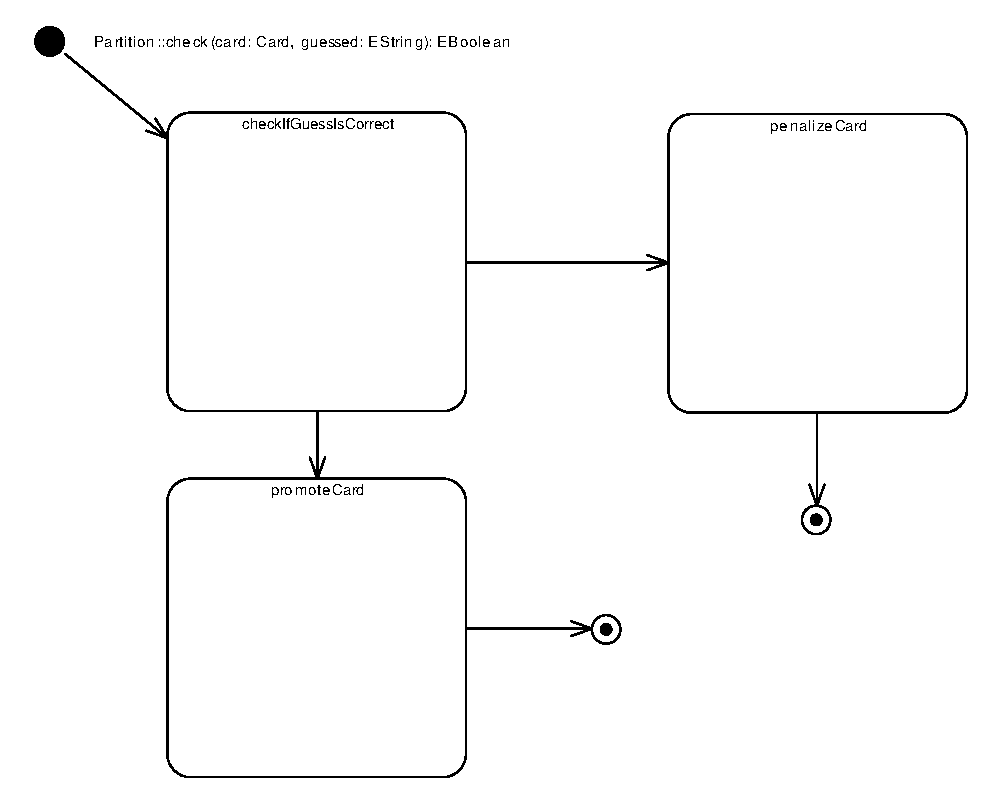
\includegraphics[width=0.9\textwidth]{ea_activityCheck}
  \caption{Activity diagram for \texttt{Partition::check}}
  \label{fig:sdm_check_start}
\end{center}
\end{figure}

\vspace{1cm}

\item[$\blacktriangleright$] In \texttt{checkCard}, create an object variable that is bound to the parameter argument, \texttt{card} 
(Fig.~\ref{fig:sdm_check_addCard}). This will represent the card the user picked from the learning box. Remember, the binding for this variable is implicitly
defined when its name is the same as the argument's name.

\begin{figure}[htbp]
\begin{center}
  \includegraphics[width=\textwidth]{ea_addObjVarCard}
  \caption{Creating the card variable}
  \label{fig:sdm_check_addCard}
\end{center}
\end{figure}

\clearpage

\item[$\blacktriangleright$] Now that the pattern has the correct card to check, it needs to compare the user's guess against the unseen \texttt{face} value on
the opposite side. To do this, we need to specify an \emph{attribute constraint}. Open the \texttt{attribute constraint} tab for \texttt{card} as depicted in
Fig.~\ref{fig:sdmcheck_att_constraint}, select the correct object attribute and operator.

\vspace{0.5cm}

\begin{figure}[htbp]
\begin{center}
  \includegraphics[width=0.6\textwidth]{ea_addAttConst}
  \caption{Creating an attribute constraint}
  \label{fig:sdmcheck_att_constraint}
\end{center}
\end{figure}

\item[$\blacktriangleright$] Similar to how the return value was specified in the previous SDM, set the \texttt{ParameterExpression} to refer to \texttt{guess}
to retrieve the user EString input. Press \texttt{Add} and admire your first attribute constraint.

\vspace{0.5cm}

Before building the other two activity nodes, let's quickly return to the control flow. Currently, the pattern will branch off into two separate patterns after
completing the initial check, then terminate the method based on whichever activity finishes first\ldots and that's not what we want at all! We need to add
\emph{edge guards}\define{Edge Guards}to change this into an \emph{if/else} construct based on the results of the comparison.

\newpage

\item[$\blacktriangleright$] To add a guard to the edge leading from \texttt{check\-If\-Guess\-Is\-Correct} to \texttt{penalize\-Card}, double click the edge
and set the \emph{Guard Type} to \texttt{Failure} (Fig.~\ref{fig:sdm_check_guard}). Repeat the process for the \texttt{Success} edge leading to
\texttt{promoteCard}.

\vspace{0.5cm}

\begin{figure}[htbp]
\begin{center}
  \includegraphics[width=0.75\textwidth]{ea_addTransitionGuard}
  \caption{Add a transition with a guard}
  \label{fig:sdm_check_guard}
\end{center}
\end{figure}

\vspace{0.5cm}

One great feature of eMolfon (with EA) provides a means of coping with large patterns.\footnote{You thought I was going to say `coping
with our coffee addiction', weren't you?} It might be nice to visualise \emph{small} story patterns directly in their nodes, but for large patterns or complex
control flow, such diagrams would get extremely cumbersome and unwieldy very quickly! This is indeed a popular argument against visual languages and it might
have already crossed your mind (``This is cute, but it'll \emph{never} scale!''). With the right tools and concepts however, even huge diagrams can be
mastered. We support \emph{extracting} story patterns into their own diagrams, and unless the pattern is really concise with 2 or 3 object variables, recommend
this course of action. In other words, eMoflon supports seprating your transformation's pattern layer from the control flow.

\vspace{0.5cm}

\item[$\blacktriangleright$] To try this, double-click the \texttt{promoteCard} story node and choose \texttt{Extract Story Pattern}
(Fig.~\ref{fig:sdm_check_extract_storypattern}). Note the new diagram that is immediately opened and created in the project browser
(Fig.~\ref{fig:sdm_new_sub_diagram}).

\begin{figure}[htbp]
\begin{center}
  \includegraphics[width=0.8\textwidth]{ea_extractStoryPattern}
  \caption{Extract a story pattern for more space and a better overview}
  \label{fig:sdm_check_extract_storypattern}
\end{center}
\end{figure}

\begin{figure}[htbp]
\begin{center}
  \includegraphics[width=0.45\textwidth]{sdm_promoteCardProjBrowser}
  \caption{A new sub diagram is created automatically}
  \label{fig:sdm_new_sub_diagram}
\end{center}
\end{figure}

\newpage

Another EA gesture you should start to take advantage of is a good ol' \emph{Drag and Drop} action from the project browser\footnote{The other two gestures we
have learnt are ``Quick Link'' and ``Quick Create''} into a diagram. We can use this move as an alternative to creating new objects (with known types) from the
SDM toolbox.

\vspace{0.5cm}

\item[$\blacktriangleright$] To create a new \texttt{Card} object variable, simply drag and drop the class from the project browser into the new (extracted)
pattern diagram (Fig.~\ref{fig:sdm_check_bound_card}).

\begin{figure}[htbp]
\begin{center}
  \includegraphics[width=\textwidth]{ea_dragDropDialogue}
  \caption{Add a new object variable per drag and drop}
  \label{fig:sdm_check_bound_card}
\end{center}
\end{figure}

\item[$\blacktriangleright$] A dialogue will appear asking what kind of variable should be created. You can create (1) a simple link (which would refer to and
be represented by \texttt{Card}'s entire class), (2) create an instance of \texttt{Card} as an object, or (3) create a subclass. Paste \texttt{Card} as an
instance and check \texttt{Autosave Selection as Default} under ``Options" so option (2) will be used next time by default. You should also check \texttt{Use
Ctrl + Mouse drag to show this Dialog}, so this dialogue doesn't appear every time. Don't worry - if you ever need options (1) and (3), you  just need to hold
\texttt{Ctrl} when dragging to invoke the dialogue then change the settings.

\item[$\blacktriangleright$] After creating the object, the same object properties dialogue will open.  Set the \texttt{Name} to \texttt{card} and its
\texttt{Binding State} to \texttt{Bound} (Fig.~\ref{fig:sdm_new_card_properties}).

\newpage

\begin{figure}[htbp]
\begin{center}
  \includegraphics[width=0.5\textwidth]{ea_addBoundObj}
  \caption{Object variable properties of the new card}
  \label{fig:sdm_new_card_properties}
\end{center}
\end{figure}

The main advantage of drag and drop is that the \texttt{Object Variable Pro\-per\-ties} dialogue should have the type of the object pre-configured. Choosing
the type in the project browser and dragging it in is (for most people) a more natural gesture than choosing the type from a long drop-down menu (as we had to
when using the SDM toolbar). This can be a great time saver for large metamodels.\footnote{Drag and drop is also possible in embedded story patterns
(still visualised in their story nodes).  You must ensure however, that the object variable is \emph{completely} contained inside the story node and does not
stick out over any edge.}

\vspace{0.5cm}

\item[$\blacktriangleright$] Currently, we have the single \texttt{card} that we want to promote through the box. Drag and drop two partition objects,
\texttt{this}, and the \texttt{nextPartition} as depicted in Fig.~\ref{fig:sdm_check_complete_sp}.

\begin{figure}[htbp]
\begin{center}
  \includegraphics[width=0.8\textwidth]{ea_promoteCardVariables}
  \caption{All object variables for story pattern \texttt{promoteCard}}
  \label{fig:sdm_check_complete_sp}
\end{center}
\end{figure}

\vspace{0.5cm}

An important point to note here is that \texttt{this} and \texttt{card} are visually differentiated from \texttt{nextPartition} by
their bold border lines. This is how we differentiate \emph{bound} from \emph{unbound} (\emph{free}) variables. We already know that matches for bound
variables are completely determined by the current context. On the other hand, matches for unbound variables, have to be determined by the pattern matcher. Such
matches are ``found'' by navigating and searching the current model for possible matches that satisfy all specified constraints (e.g. type of the variable,
links connecting it to other variables and attribute constraints). In our case, the next partition will have to be determined by navigating from \texttt{this}
via the \texttt{next} link in the metamodel.

\vspace{0.5cm}

\item[$\blacktriangleright$] Quick link from \texttt{this} to \texttt{nextPartition} (or vice-versa) to create a \texttt{next} link variable, as shown in
Fig.~\ref{fig:sdm_check_link_variable}. As you can see, there are several more property options. The goal is to have the current partition to proceed or point
to the \texttt{nextPartition} via the \texttt{next} reference, so select the second option. This will cause the reference to be defined in \texttt{this}.
Alternatively, you could define the reference in \texttt{nextPartition} by setting the link proceed from the next partition into the \texttt{previous}
partition, \texttt{this}.

\begin{figure}[htbp]
\begin{center}
  \includegraphics[width=0.85\textwidth]{ea_promoteLinkProperties}
  \caption{Connecting \texttt{this} and \texttt{nextPartition}}
  \label{fig:sdm_check_link_variable}
\end{center}
\end{figure}

\vspace{0.5cm}

\item[$\blacktriangleright$] Continue creating links between \texttt{card} and each partition. Remember - you want to \emph{destroy} the reference to
\texttt{this}, and \emph{create} a new connection to \texttt{nextPartition}. If everything is set up correctly, \texttt{promoteCard} should now closely resemble
Fig.~\ref{fig:sdm_check_complete_activity_node}.

\begin{figure}[htbp]
\begin{center}
  \includegraphics[width=0.8\textwidth]{ea_promoteCardCompleted}
  \caption{Complete story pattern for \texttt{promoteCard}}
  \label{fig:sdm_check_complete_activity_node}
\end{center}
\end{figure}

\clearpage

\item[$\blacktriangleright$] Double click the anchor in the top left corner and repeat the process for \texttt{penalizeCard}: First extract the story pattern,
then create the necessary variables and links as depicted in Fig.~\ref{fig:sdm_check_complete_penalize}. As you can see, this pattern is nearly identical to
\texttt{promoteCard}, except it moves the card to a \texttt{previousPartition}.

\vspace{0.5cm}

\begin{figure}[htbp]
\begin{center}
  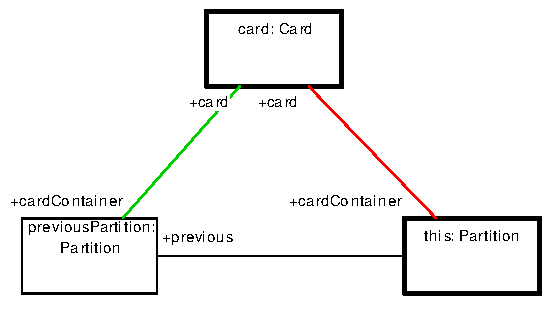
\includegraphics[width=0.8\textwidth]{ea_completeActivityPenalize.pdf}
  \caption{Story pattern for activity node \texttt{penalizeCard}}
  \label{fig:sdm_check_complete_penalize}
\end{center}
\end{figure}


\vspace{0.5cm}

To complete the \texttt{check} SDM, we need to signal (as a return value) the result of the check - was the card promoted or penalised? To do this, we need to
edit the stop nodes so they return a\define{LiteralExpression}\emph{LiteralExpression}. This expression type can be used to specify arbitrary text, but
should really only used for true literals like 42, ``foo'' or \texttt{true}. It can be (mis)used for formulating any (Java) expression that will simply be
transferred ``literally'' into the generated code, but this is obviously sort of dirty\footnote{It defeats, for example, any attempt to guarantee type safety}
and should be avoided when possible.

\vspace{0.5cm}

\item[$\blacktriangleright$] To implement a literal, double click the stop node stemming from  \texttt{promoteCard}, and change the expression type from
\texttt{void} to \texttt{LiteralEx\-pression} (Fig.~\ref{fig:sdm_check_literal_exp}). Change the value in the window below to \texttt{true}. Press \texttt{OK},
then finish the SDM by returning \texttt{false} after \texttt{penaliseCard} in the same manner. Your diagram should now resemble
Fig.~\ref{fig:sdm_check_finish}.

\begin{figure}[htbp]
\begin{center}
  \includegraphics[width=0.5\textwidth]{ea_stopNodeLiteral}
  \caption{Add a return value with a literal expression}
  \label{fig:sdm_check_literal_exp}
\end{center}
\end{figure}

\begin{figure}[htbp]
\begin{center}
  \includegraphics[width=\textwidth]{ea_sdmCheckComplete}
  \caption{Complete SDM for \texttt{Partition::check}}
  \label{fig:sdm_check_finish}
\end{center}
\end{figure}

\clearpage

\item[$\blacktriangleright$] Great job - the SDM is now complete! Validate and export your project, then inspect the implementation code for \texttt{check}. We
strongly recommend that you even write a simple JUnit test (take a look at our simple test case from Part I for inspiration) to take your brand new SDM for a
test-spin.

\item[$\blacktriangleright$] To see how this is implemented in the textual syntax, see Figs. \ref{fig:completedPatterns} and \ref{fig:finalMethod} in the
following section.

\jumpSingle{sec:emptyPartition}

\end{itemize}



\newpage
\section{Emptying a partition of all cards}
\genHeader
\hypertarget{sec:emptyPartition}{}

This next SDM should \emph{empty} a partition by removing every card contained inside. Since we can assume that there is more than one card in the
partition\footnote{If there was only one, we would just invoke \texttt{removeCard}.}, we obviously need some construct for repeatedly deleting each card in the
partition an unknown number of times (Fig.~\ref{fig:goal_empty}). 

\vspace{0.5cm}

\begin{figure}[htbp]
	\centering
  \includegraphics[width=0.3\textwidth]{goal_partitionEmpty.pdf}
	\caption{Emptying a partition of every card}
	\label{fig:goal_empty}
\end{figure}
\FloatBarrier

\vspace{0.5cm}

In SDM, this \define{For Each} construct is accomplished via a \emph{for each} story node. A
\emph{for each} story node performs the specified actions for \emph{every} match in its pattern. That means for every \texttt{Card} the pattern finds, it'll
perform an action set.

This construct however, gives us two very interesting points to discuss. Firstly, how would the pattern be interpreted if the node was a normal story node, not
a \emph{for each}?

The pattern would specify that \emph{a} card should be matched and deleted from the current partition - that's it. The \emph{exact} card is not specified,
meaning that the actual choice of the card is \emph{non-deterministic} or random, and it is only done once. This randomness is a common property of both graph
transformations and pattern matching, and it's something that takes time getting used to.  In general, there are no guarantees concerning the choice and
order of valid matches. The \emph{for each} node ensures that \emph{all} cards will be matched and deleted.

Our second point is determining if we actually need to destroy the link between \texttt{this} and \texttt{card}. Would the pattern be interpreted differently if we
destroyed \texttt{card} and left the link?

The answer is no, the pattern would yield the same result, regardless of if the link is explicitly destroyed!  \define{Dangling Edges}This is due to the
transformation engine eMoflon uses\footnote{CodeGen2, a part of Fujaba \url{http://www.fujaba.de/}}. It ensures that there are never any \emph{dangling edges}
in a model. Since deleting just the \texttt{card} would result in a `dangling edge' attached to \texttt{this}, that link is deleted as well. Explicitly
destroying the link is therefore a matter of taste, so \ldots why not be as explicit as possible?

\fancyfoot[R]{ $\triangleright$ \hyperlink{emptyPartition vis}{Next [visual]\hspace{0.2cm} } \\ $\triangleright$ \hyperlink{emptyPartition tex}{Next [textual]} }

\newpage
\hypertarget{emptyPartition vis}{}
\subsection{Implementing empty}
\visHeader

\begin{itemize}

\item[$\blacktriangleright$] Open a new activity diagram for \texttt{Partition.empty}. To begin building the \emph{for each} pattern, quick create a new story
node and edit its properties. Name it \texttt{deleteCardsInPartition} and change the \texttt{Type} from \texttt{StoryNode} to \texttt{ForEach}. You'll also want
to create the invoking \texttt{Partition} object, so ensure that too, is selected. As you can see, a \emph{for each} node is represented as a stacked node to
indicate the potential for repetition.

\begin{figure}[htbp]
\begin{center}
  \includegraphics[width=0.9\textwidth]{ea_sdmEmptyNew}
  \caption{Creating a looping story node}  
  \label{fig:sdm_foreach}
\end{center}
\end{figure}

\item[$\blacktriangleright$] Now create the neccessary \texttt{card} variable needed to complete this SDM. Unlike \texttt{removeCard}\footnote{See
Fig.~\ref{fig:sdm_complete_control_flow}} however, the goal of \texttt{emptyCards} is not just to remove the link between the selected partition and card, we
want the matched \texttt{card} to be \emph{completely} deleted. This means in the properties tab, after setting the name and binding state, you'll need to set
the \texttt{Binding Operator} to \texttt{Destroy} (Fig.~\ref{fig:sdm_bindingOperator}).

\item[$\blacktriangleright$] Complete the story pattern as indicated in Fig.~\ref{fig:sdm_end}. Notice that the guard that terminates the looping node has an
\texttt{[end]} edge guard. Indeed, a \emph{for each} story node \emph{must} execute an \texttt{end} activity when all matches in the pattern have been
handled. \texttt{empty} is defined as a \texttt{void} method, so don't worry about setting any return values.

\begin{figure}[htbp]
\begin{center}
  \includegraphics[width=0.65\textwidth]{ea_emptyBindingOperator}
  \caption{Editing \texttt{card} so the variable gets destroyed}  
  \label{fig:sdm_bindingOperator}
\end{center}
\end{figure}

\begin{figure}[htbp]
\begin{center}
  \includegraphics[width=0.8\textwidth]{ea_sdmEmptyComplete}
  \caption{Completed \texttt{empty} story pattern}  
  \label{fig:sdm_end}
\end{center}
\end{figure}
\FloatBarrier

\item[$\blacktriangleright$] Done! You've now learnt that in order to create a repeating action, all you need to do is change a standard standard story node
into a \texttt{for each} node, and include \emph{edge guards}. Inspect Fig.~\ref{fig:emptyControlFlow} and Fig.~\ref{fig:emptyPattern} to see how this is
implemented in the textual specifications.

\fancyfoot[R]{ $\triangleright$ \hyperlink{sec:invertCard}{Next}} 

\end{itemize}



\newpage
\subsection{Textual; emptying}
\texHeader
\hypertarget{emptyPartition tex}{}

\texttt{}
\emph{}

\begin{itemize}
 
\item[$\blacktriangleright$] Can use type completion here to set up the flow for your for each. Press ctrl space and select forEach

\item[$\blacktriangleright$] create a \texttt{deleteCardsInPartition} pattern. While similar to \texttt{removeCard}, this goes one step further by requesting a
full deletion/destruction of card. This means we need to destroy the obj. variable. Work until your workspace resembles (Fig).

\item[$\blacktriangleright$] That's it! Check out how it's done in the visual syntax.

\end{itemize}



\newpage
\hypertarget{sec:invertCard}{}
\section{Inverting a card}
\genHeader

This next SDM \emph{inverts} a card by swapping its back and face values (Fig.~\ref{fig:goal_invert}). This therefore ``turns a card around'' in the learning
box. This action makes sense if a user wants to try learning, for example, the definition of a word in the other (target) language. Instead of guessing the
definition of every word when presented with the term, perhaps they would like to guess the term when presented with the definition. This method doesn't need to
accept any parameters -- it'll use a bound \texttt{this} object variable.

\vspace{0.5cm}

\begin{figure}[htbp]
	\centering
    \includegraphics[width=0.4\textwidth]{goal_invert.pdf}
 	\caption{Inverting the attributes of a \texttt{Card}}
 	\label{fig:goal_invert}
\end{figure}
\FloatBarrier

Something new that we'll use in this SDM are \emph{assignments}\define{Assignments} to set the attributes of a \texttt{temp} object variable with \texttt{card},
then again to actually swap the \texttt{card} values. An assignment is simply an attribute constraint\footnote{Which we first encountered in \texttt{check}}
with a \texttt{`:='} operator. Though it may be slightly confusing to refer to an assignment as a constraint, if you think about it, \emph{everything} can be
considered as a constraint that must be fulfilled using different strategies.

With \texttt{invert}, a successful match is achieved not by searching as you would with a comparison (\texttt{==, >, <, \ldots}), but by \emph{performing} the
above assignment. If the assignment cannot be completed, the match is invalid. Similarly, non-context elements (set to create or destroy) can be viewed as
structural constraints that are fulfilled when the corresponding element is created or destroyed.  A constraint is therefore a unifying concept similar to
``everything is an object'' from OO, and ``everything is a model'' from metamodelling.  If you're interested in why \emph{unification} is considered cool, check
out~\cite{BEZ05}.

\newpage
\subsection{Implementing invert}
\visHeader
\hypertarget{invertCard vis}{}

\begin{itemize}

% Make sure you explain how/why the green box. Hasn't been convered yet
\item[$\blacktriangleright$] Model the SDM depicted in Fig.~\ref{fig:sdm_invert}. Remember, the green creational object variable is made by setting the binding
operator as \texttt{create}.

% Explain how to use the new assignments??

\vspace{1cm}

\begin{figure}[htbp]
\begin{center}
  \includegraphics[width=0.9\textwidth]{ea_swappingCard.pdf}
  \caption{Swap back and face of the card}  
  \label{fig:sdm_invert}
\end{center}
\end{figure}

\item[$\blacktriangleright$] Believe or not, that's it! Check out how this method was implemented in the textual syntax by reviewing
Fig.~\ref{fig:invertPatterns} in the next section.

\end{itemize}


\newpage
\subsubsection{Inversion review}
\genHeader
\hypertarget{invert close}{}

Before we start the next SDM, let's quickly review one point. Have you considered why the \texttt{temp} object variable is bound in the second pattern for
\texttt{invert}, (\texttt{swap variables}), but not where it's first defined in \texttt{initialize temp}?\footnote{See Fig.~\ref{ea:sdm_invertComplete}
(Visual) or Fig.~\ref{eclipse:invertPatterns} (Textual)} This is a new case for bound variables that we haven't treated yet!

Until now, we have seen object variables that can be bound to (1) an argument of the method (set when the method is invoked), or (2) the
current object (\texttt{this}) whose method is invoked. In both cases, the object to be matched is completely determined by the context of the method before
the pattern matcher starts. This means that it does not need to be determined or found by the pattern matcher.

Setting \texttt{temp} as bound in \texttt{Swap variables} is a third case in which an object variable is bound to a value determined in a \emph{previous}
activity node without using a special expression type. In this SDM, this means \texttt{temp} will be bound to the value determined for a variable
of the same name in the previous node, \texttt{Initialize temp}. This binding feature enables you to refer to previous matches for object variables in the
preceding control flow.

On a separate note, you're just over halfway through completing this part of the eMoflon handbook, so give your brain a small break. Take a walk, pour
yourself another coffee, and check out one of my favourite jokes:
\syntax{How do you wake up Lady Gaga?}

\vspace{0.5cm}

\syntax{Poke her face!}




\newpage
\section{Growing the box}
\genHeader

In this SDM, we shall explicitly specify how our learning box is to be built up. We create a specific pattern that will append new partition elements
to the end of \texttt{Box} which will follow our established movement rules (Fig.~\ref{fig:membox_depiction}) for a \texttt{Card}. This means the new partition
will become the \texttt{next} reference of the absolute last partition, and its \texttt{previous} reference must connect to the absolute first partition in the
box (Fig.~\ref{fig:goal_grow}).

\begin{figure}[htbp]
 	\centering
  	\includegraphics[width=0.7\textwidth]{growBoxNACGoal.pdf}
	\caption{Growing a box by inserting a new partition}
	\label{fig:goal_grow}
\end{figure}
\FloatBarrier

Unfortunately, precise instructions such as these contradict the pattern matcher. We know that, no matter what, a box will always be able to
define first and last partitions. As explained in \hyperlink{sec:emptyPartition}{section 5} however, these will be determined non-deterministically. They will
be chosen at random, and are unlikely to be the actual first and last partitions. How can we guarantee this match to be true?

SDMs provide a declarative means of identifying specific partitions via \emph{Negative Application Conditions}, simply referred to as
\mbox{NAC}s.\footnote{Pronounced $\backslash 'nak \backslash$}\define{NAC}\mbox{NAC}s express structures that are forbidden to exist before or after applying a
transformation rule. In this SDM, the \mbox{NAC} will be a link variable that may not be valid during the pattern match. In the theory of algebraic
graph transformations \cite{EEPT06}, \mbox{NACs} can be complex graphs that are much more general and powerful but in our implementation,\footnote{To be
precise, in CodeGen2 from Fujaba} we only support single negative elements (object or link variables).

As depicted in Fig.~\ref{fig:goal_grow}, to create an appropriate \mbox{NAC} that constrains possible matches, we'll need to check to see if the current matched
pattern has certain `active' link variables. Suppose the targeted last partition has a set \texttt{next} reference. This means it is \emph{not} the absolute
last partition, and so the match becomes invalid. We only want the pattern to insert a new partition when the \texttt{next} link is null. Similarly, if the
targeted first partition has a \texttt{previous} value, the match is invalid. The complete pattern match is therefore made unique through NACs and thus becomes
\emph{deterministic} by construction. In other words, if you \emph{grow} the box with this method, there will always be exactly one first and one last
partition.

Of course, to complete this method we will still need to determine how \emph{many} partitions to add! Since the new size must be calculated depending on the
rest of the partitions currently in the box (partitions usually get bigger) we'll need to call a helper method, \texttt{determineNextSize()}. Due to the
low-level nature of this method however, it will be easier to implement this via \emph{Injections}, rather than an SDM.


Previously,\footnote{See Part II, section 5} we learned how to write handwritten code in an implementation file, then generate
a \emph{partial class} to inject code into the metamodel. Now however, we'll generate and edit a partial class to automatically insert code into the
corresponding Java file, which will then inject it into the metamodel.

\begin{itemize}

\item[$\blacktriangleright$] Go to ``BoxImpl.java'' and, without editing any method signatures there, generate its corresponding injection file by either right
clicking the file in the package explorer or within the editor window (Fig.~\ref{}).

\item[$\blacktriangleright$] A second file should now be placed in the \texttt{injection} folder. Open \texttt{BoxImpl.inject} and notice the
partial class includes every method declaration but (as expected) no implementation code (Fig.~\ref{fig:injection_partialClassBox}).

\begin{figure}[htbp]
    \centering
    \includegraphics[width=1.0\textwidth]{eclipse_injectionBoxImpl}
    \caption{Generated Injection file for \texttt{BoxImpl.java}}
    \label{fig:injection_partialClassBox}
\end{figure}

\item[$\blacktriangleright$] Complete the \texttt{addToStringRep} and \texttt{determineNextSize} methods as specified in Fig.~\ref{code:complete_inject_file}
below.\footnote{Note: To help avoid errors, this text is able to be copied and pasted}

\vspace{0.5cm}

\begin{figure}[htbp]
        \centering
        \begin{lstlisting}[language=Java, keywordstyle={\bfseries\color{purple}}, backgroundcolor=\color{white}]
    @model addToStringRep (Card card) <--

            StringBuilder sb = new StringBuilder();

            if (stringRep == null)
            {
                sb.append("BoxContent: [");

            }
            else
            {
                sb.append(stringRep);
                sb.append(", [");
            }

            sb.append(card.getFace());
            sb.append(", ");
            sb.append(card.getBack());
            sb.append("]");

            stringRep = sb.toString();
    -->

    @model determineNextSize () <--

            return getContainedPartition().size() * 10;
    -->

        \end{lstlisting}
        \caption{Implementation of helper methods as an injection}
        \label{code:complete_inject_file}
    \end{figure}
    \FloatBarrier

\vspace{0.5cm}

\item[$\blacktriangleright$] Right-click the injection file, and rebuild your project by selecting ``eMoflon/Clean and
Build''(Fig~\ref{fig:eclipse_buildFromInjecton}).

\item[$\blacktriangleright$] The helper methods should now be implemented in \texttt{BoxImpl.java}, which can be found under
the ``/gen/LearningBoxLanguage.impl'' package (Fig~\ref{fig:eclipse_updatedBoxImpl}).

\item[$\blacktriangleright$] For additional information on injections, check out Part IV: Miscellaneous. Be sure to also
review the work we completed with injections in Part II: Ecore.

\newpage

\vspace*{2cm}

\begin{figure}[htbp]
    \centering
    \includegraphics[width=\textwidth]{eclipse_buildFromInject}
    \caption{Build the entire project from the injection file}
    \label{fig:eclipse_buildFromInjecton}
\end{figure}

\newpage

\vspace*{2cm}

\begin{figure}[htbp]
    \centering
    \includegraphics[width=\textwidth]{eclipse_updatedBoxImpl}
    \caption{Updated \texttt{BoxImpl.java} file}
    \label{fig:eclipse_updatedBoxImpl}
\end{figure}

\fancyfoot[R]{ $\triangleright$ \hyperlink{growBox vis}{Next [visual]\hspace{0.2cm} } \\ $\triangleright$ \hyperlink{growBox tex}{Next [textual]} }

\end{itemize}


\newpage
\hypertarget{growBox vis}{}
\subsection{Implementing grow}
\visHeader

\begin{itemize}
 
\item[$\blacktriangleright$] Start by creating the simple story pattern depicted in Fig.~\ref{fig:sdm_grow_1}. This matches the box, \texttt{this}, with
\emph{any} two partitions.\footnote{Remember, the \emph{pattern matcher} is randomized!}

\vspace{0.5cm}

\begin{figure}[htbp]
\begin{center}
  \includegraphics[width=\textwidth]{ea_elementsGrowBox}
  \caption{Context elements for SDM}  
  \label{fig:sdm_grow_1}
\end{center}
\end{figure}

\item[$\blacktriangleright$] To create an appropriate \mbox{NAC} to constrain the possible matches for \texttt{lastPartitionInBox},  create a new
\texttt{Partition} object variable \texttt{nextPartition} and set\define{Binding\\Semantics}its \emph{binding semantics} to \texttt{negative}
(Fig.~\ref{fig:sdm_grow_2}). The object variable should be visualised as being cancelled or struck out. 
 
\begin{figure}[htbp]
\begin{center}
  \includegraphics[width=0.7\textwidth]{ea_newNac}
  \caption{Adding a negative element}  
  \label{fig:sdm_grow_2}
\end{center}
\end{figure}
 
\item[$\blacktriangleright$] Now, quick link \texttt{nextPartition} to \texttt{lastPartitionInBox}. Be sure choose the link type carefully! The
\texttt{nextPartition} should play the role of \texttt{next} with respect to \texttt{lastPartitionInBox}. This combination (the negative binding and reference)
tells the pattern matcher that if the (assumed) last partition has an element connected to its \texttt{next} reference, the current match is invalid.

\item[$\blacktriangleright$] Great work -- the first NAC is complete! In a similar fashion, create the remaining NAC for \texttt{firstPartitionInBox}. Name the
negative element \texttt{previousPartition}, and again, be sure to double-check the navigation.

\item[$\blacktriangleright$] Finally, complete the pattern rule so that it closely resembles Fig.~\ref{fig:sdm_grow_3}. 

\begin{figure}[htbp]
\begin{center}
  \includegraphics[width=\textwidth]{ea_NACComplete} 
  \caption{Determining the first and last partitions with NACs}  
  \label{fig:sdm_grow_3}
\end{center}
\end{figure}
 
\item[$\blacktriangleright$] Notice how the created partition \texttt{newPartition} is `hung' into the box. It becomes the next partition of the current
\emph{last} partition, and its previous partition is automatically set to the first partition in the box (as dictated by the rules set in
Fig.~\ref{fig:membox_depiction}). In other words, the new partition is appended onto the current order of partitions.

\item[$\blacktriangleright$] In order to complete \texttt{grow}, we need to set the size of the \texttt{newPartition}. Given that the new size is calculated
via the helper function \texttt{det\-er\-mine\-Next\-Size}, we need to invoke a \emph{MethodCallExpression}.\define{MethodCallExpression}A MethodCallExpression
is another specialized EA mechanism. As the name suggests, its designed to access any method defined in any class of the current project. Go ahead and invoke
the corresponding dialogue to activate the assignment (\texttt{:=}) operator, and match your values to Fig.~\ref{fig:sdm_grow_4}
 
\begin{figure}[htbp]
\begin{center}
  \includegraphics[width=0.6\textwidth]{ea_attributeMethodCall.png}
  \caption{Invoking a method via a \texttt{MethodCallExpression}}  
  \label{fig:sdm_grow_4} 
\end{center}
\end{figure}

Since \texttt{determineNextSize} doesn't require any parameters, you can ignore the \texttt{Parameter values} field this time. For future reference however,
parameters can be specified by choosing the appropriate parameter declaration between guillemets (e.g. \texttt{<Box box>}) found in the drop-down menu and typing in the
value (this is basically a literal expression). Don't forget to press the \texttt{Save} button for every parameter, then \texttt{Add} + \texttt{OK} to confirm
and close the dialogue.

\vspace{0.5cm}

\item[$\blacktriangleright$] If you've done everything right, your SDM should now closely resemble Fig.~\ref{fig:growComplete}. As usual, try to export,
generate code, and inspect the method implementation.

\vspace{0.5cm}

\item[$\blacktriangleright$]  That's it - your \texttt{grow} SDM is complete! This was probably the most challenging SDM to build, so give yourself a solid 
pat on the back. If you found it easy, well then \ldots I don't think I'm doing my job correctly. To see how this is done in the texual syntax, review
Fig.~\ref{fig:patternComplete}.\footnote{We do recommend reading the instructions for this one, since NACs can be tricky}

\vspace{0.5cm}

\begin{figure}[htbp]
\begin{center}
  \includegraphics[width=\textwidth]{ea_growFinal}
  \caption{Complete SDM for \texttt{Box::grow}}  
  \label{fig:growComplete}
\end{center}
\end{figure}
\FloatBarrier

\jumpSingle{sec:stringRep}

\end{itemize}


\clearpage
\hypertarget{growBox tex}{}
\subsection{Implementing grow}
\texHeader

\vspace*{0.5cm}

\begin{itemize}

\item[$\blacktriangleright$] In \texttt{grow}, create a simple control flow with one story pattern. You'll want this pattern to match the invocation box with
\emph{any} two partitions, so create a bound \texttt{this} box, and free \texttt{firstPartitionInBox} and \texttt{lastPartitionInBox} partitions.
You'll also need a variable set to create to represent the new partition. The skeleton of your pattern should now resemble (Fig.~\ref{fig:growPattSkel}).

\vspace{0.5cm}

\begin{figure}[htbp]
\begin{center}
  \includegraphics[width=0.5\textwidth]{eclipse_growPatternSkeleton}
  \caption{addPartitionsBox.pattern skeleton}
  \label{fig:growPattSkel}
\end{center}
\end{figure}

\item[$\blacktriangleright$] Next, we need to create an appropriate \emph{NAC} which will constrain the possible choices for \texttt{lastPartitionInBox}.
Create a \texttt{nextPartition} variable with an `!' operator (negation) preceding it immediately below \texttt{last\-Part\-it\-ion\-In\-Box}.

\vspace{0.5cm}

\item[$\blacktriangleright$] Now add \texttt{-> next : nextPartition} the the \texttt{lastPartition} scope. This
command will attempt to establish a \texttt{next} link from the last partition. Next, add \texttt{++ -> next: newPartition} (Fig.~\ref{fig:firstNAC}).
This line will only be reachable if the NAC fails! It establishes the \texttt{newPartition} as the final partition.

\begin{figure}[htbp]
\begin{center}
  \includegraphics[width=0.5\textwidth]{eclipse_growLastNAC}
  \caption{Creating the first NAC}
  \label{fig:firstNAC}
\end{center}
\end{figure}

\vspace{0.5cm}

\item[$\blacktriangleright$] In a similar fashion, create a second NAC, \texttt{previousPartition}, for \texttt{firstPartitionInBox}. No new references have to
be created here, so all you need to establish is the link connecting \texttt{firstPartitionInBox} to the negative element, \texttt{previousPartition}.

\begin{figure}[htp]
\begin{center}
  \includegraphics[width=0.55\textwidth]{eclipse_growFirstNAC}
  \caption{Pattern now with both NACs}
  \label{fig:growPatt}
\end{center}
\end{figure}

\clearpage

\item[$\blacktriangleright$] Connect \texttt{@this} with appropriate links to the first and last partitions, then establish the \texttt{box} and
\texttt{previous} references in \texttt{newPartition} (Fig~\ref{fig:growAllLinks}).

\vspace{0.5cm}

\begin{figure}[htp]
\begin{center}
  \includegraphics[width=0.65\textwidth]{eclipse_growLinks}
  \caption{A complete \emph{deterministic} pattern match}
  \label{fig:growAllLinks}
\end{center}
\end{figure}

\item[$\blacktriangleright$] \update explain the assumed `++'

\item[$\blacktriangleright$] We're not \emph{quite} done yet - our newest partition doesn't yet have a size. This means that not only do we need to make
another attribute contsraint, but \texttt{newPartition} needs to invoke a method in order to get the correct value. Call the method as you would in Java. 
Your workspace should then resemble Fig.~\ref{fig:patternComplete}.

\begin{figure}[htp]
\begin{center}
  \includegraphics[width=0.9\textwidth]{eclipse_growFinished}
  \caption{Complete pattern for adding a new \texttt{partition} to \texttt{Box}}
  \label{fig:patternComplete}
\end{center}
\end{figure}

\vspace{0.5cm}

\item[$\blacktriangleright$] That's all! While NACs may be difficult to understand at first, as you can see, they're not hard to implement, and
can be used in a wide variety of applications. To see how this method is implemented in the visual syntax, check out Fig~\ref{fig:growComplete} from the previous
section.

\item[$\blacktriangleright$] \update	move branching content here (to complete grow)

\end{itemize}


\newpage
\hypertarget{sec:stringRep}{}
\section{String representations}
\genHeader

In the next SDM we shall create a string representation for all the contents in a single learning box. To accomplish this, we will have to iterate through 
every card, in every partition. The concept is similar to \texttt{Partition}'s \texttt{empty} method, except we'll need to create a nested \emph{for each}
loop (Fig.~\ref{fig:goal_stringRep}). Further still, we'll need to call a helper method to add the contents of each card to \texttt{stringRep}.

\vspace{1cm}

\begin{figure}[htbp]
	\centering
	\includegraphics[width=0.3\textwidth]{goal_stringRep.pdf}
	\caption{Nested \emph{For Each} loops}
	\label{fig:goal_stringRep}
\end{figure}

\vspace{1cm}

As you can see, The first loop will match all partitions, while the second matches each card. For each card, a \emph{statement} is used to invoke the
\texttt{addToStringRep()} method.

\vspace{0.5cm}

While we declared \texttt{addToStringRep()} in Part II, we didn't implement it. Analogously to how you implemented \texttt{determineNextSize} in the
previous section, quickly edit \texttt{BoxImpl.java} again with the code in Fig.~\ref{code:addToStringRep_inject_file} and rebuild your
project. Confirm the changes in \texttt{BoxImpl.inject}, and you'll be ready to start.

\newpage

\vspace*{3cm}

\begin{figure}[h!]
        \centering
        \begin{lstlisting}[language=Java, keywordstyle={\bfseries\color{purple}}, backgroundcolor=\color{white}]
		public void addToStringRep(Card card) {
			// [user code injected with eMoflon]
			StringBuilder sb = new StringBuilder();
			if (stringRep == null) {
				sb.append("BoxContent: [");
			} else {
				sb.append(stringRep);
				sb.append(", [");
			}
			sb.append(card.getFace());
			sb.append(", ");
			sb.append(card.getBack());
			sb.append("]");
			stringRep = sb.toString();
	}
        \end{lstlisting}
        \caption{Editing box.impl again}
        \label{code:addToStringRep_inject_file}
    \end{figure}
    \FloatBarrier

\jumpDual{stringRep vis}{stringRep tex}

\newpage
\subsection{Visual; String Representation}
\visHeader
\hypertarget{stringRep vis}{}

SDMs support arbitrary nesting of For Each story nodes via special guards. In \hyperlink{emptyPartition vis}{section 5.1} 
we already used the \texttt{[end]} edge guard to terminate a loop and, as depicted in \note{[each time]}Fig.~\ref{fig:sdm_tostring_1}, an
\texttt{[each time]} guard is used to indicate control flow that is \emph{nested} in the For Each story node and is executed for each match.

\begin{itemize}

\item[$\blacktriangleright$] Go ahead and create the SDM for \texttt{Box::toString} until it closely resembles Fig.~\ref{fig:sdm_tostring_1}. Don't forget to
create the new \emph{[each time]} guards. Note that \texttt{partition} in \texttt{ForAllCards} is bound  and thus refers to the assigned value determined in
\texttt{ForAllParitions}.

\vspace{0.5cm}

\begin{figure}[htbp]
\begin{center}
  \includegraphics[width=0.8\textwidth]{ea_nestedControl.pdf}
  \caption{Control flow with nested loops} 
  \label{fig:sdm_tostring_1}
\end{center}
\end{figure}

\clearpage

\item[$\blacktriangleright$] To actually do something sensible with each card, double-click the empty activity node that is taken each time a card is matched and invoke the \texttt{Edit
ActivityNode} dialogue. Now choose \texttt{addToStringRep} as the name, and \texttt{StatementNode} as the type of the activity node
(Fig.~\ref{fig:sdm_tostring_2}). \note{Statement Nodes} A statement node is used to invoke a method from a class in any package in the current EA project via a
MethodCallExpression. This way, the method invocation is represented as an activity node and is guaranteed to be executed at this point in the control flow.

\begin{figure}[htbp]
\begin{center}
  \includegraphics[width=0.8\textwidth]{ea_createStatementNode.png}
  \caption{Invoking a method in a \texttt{StatementNode}}  
  \label{fig:sdm_tostring_2}
\end{center}
\end{figure}

\item[$\blacktriangleright$] As we have already used a MethodCallExpression in an attribute constraint (\hyperlink{sec:growBox}{Sec. 5}), go ahead and click the
\texttt{Method Call Expression} tab and select \texttt{MethodCallExpression} as expression, \texttt{this} as target, \texttt{addToStringRep} as operation and
\texttt{card} as value of the parameter. That way, we pass the object variable \texttt{card} to the method
\texttt{addToStringRep} as parameter.

Statement nodes should be used to interact with methods that are implemented by hand and provide a means of invoking libraries and arbitrary Java code from
SDMs. Please note that we do not differentiate at this point between methods that are implemented via an SDM or by hand and thus, statement nodes can of course
be used to invoke other SDMs via a MethodCallExpression. Most importantly, this enables \emph{recursion} as the current SDM can be invoked on \texttt{this} with
appropriate new arguments.

A final point to note is that the return value of the method is ignored -- statement nodes are therefore best used for void methods that either have appropriate
side effects (e.g. manipulate their arguments). We shall learn in a few pages how to invoke methods with non-primitive return values (if a method returns a
primitive then it can be invoked in an attribute constraint as in \hyperlink{sec:growBox}{Sec. 5}). % Double check w/original!

% \begin{figure}[htbp]
% \begin{center}
%   \includegraphics[width=0.4\textwidth]{pics/sdmBilder/toString/sdm74.png}
%   \caption{Specify a \texttt{MethodCallExpression} in the
%   \texttt{StatementNode}}
%   \label{fig:sdm_tostring_3}
% \end{center}
% \end{figure}

\item[$\blacktriangleright$] To complete the SDM, return the final string representation of the box via an \texttt{AttributeValueExpression} in the stop node
(Fig.~\ref{fig:sdm_tostring_4}).


\begin{figure}[ht]
   \centering
      \subfloat[Specify a \texttt{MethodCallExpression} in the \texttt{StatementNode}]{
        \includegraphics[width=0.4\textwidth]{sdm74}
      }\qquad
      \subfloat[Using a \texttt{AttributeValueExpression} as a return value]{
        \includegraphics[width=0.45\textwidth]{sdm75}
        \label{fig:sdm_tostring_4}
      }
      \caption{}
\end{figure}
\FloatBarrier

% \begin{figure}[htbp]
% \begin{center}
%   \includegraphics[width=0.5\textwidth]{pics/sdmBilder/toString/sdm75.png}
%   \caption{Using a \texttt{AttributeValueExpression} as a return value.}  
%   \label{fig:sdm_tostring_4}
% \end{center}
% \end{figure}

Take some time to compare and reflect on the complete SDM as depicted in Fig.~\ref{fig:sdm_tostring_5}.  The idea was to abstract from the actual text
representation of the box and model the necessary traversal of the data structure. The helper methods \texttt{addToStringRep}could, for example, build up a
string buffer and update this string representation. While modelling this SDM, we have seen that for each story nodes can be nested, and have learnt two new
uses of MethodCallExpressions that provide a type safe\footnote{Apart from the literal expressions used for specifying argument values.} means of invoking
methods from SDMs.

\begin{figure}[htbp]
\begin{center}
  \includegraphics[width=0.75\textwidth]{ea_completeActivityStringRep.pdf}
  \caption{The complete SDM for \texttt{Box::toString}}  
  \label{fig:sdm_tostring_5}
\end{center}
\end{figure}
\FloatBarrier

\end{itemize}


\newpage
\subsection{Textual; String Representation}
\texHeader
\hypertarget{stringRep tex}{}

Fill


\newpage
\section{Fast cards!}
\genHeader
\hypertarget{sec:fastCard}{}

Congratulations, you're almost there! This is the last SDM needed before your Leitner's learning box is fully functional.

For very simple cards (i.e: words in different language that are similar), it might be a bit annoying to have to answer these cards again and again in
successive partitions. Such \emph{fast} cards should somehow be marked and handled differently. If a fast card is correctly answered once, it should be
immediately moved to the final partition in the box. This way, the card is practiced once, and only tested once more before finally being ejected from the
box.

It makes sense that a \texttt{FastCard} element inherits a \texttt{Card}, so we'll extend the current object in our metamodel in a new eclass, which will create
a marker to show it behaves differently (Fig.~\ref{fig:goal_fastCard}).

\begin{figure}[htbp]
	\centering
    \includegraphics[width=0.7\textwidth]{goal_fastCard}
	\caption{Checking a fast card against a guess}
	\label{fig:goal_fastCard}
\end{figure}
\FloatBarrier

In addition to creating a new \texttt{eclass}, we also need to extend the existing \texttt{check} method to check for this special card type once a guess is
determined to be correct. Now \texttt{check} needs to decide, based on the dynamic type\footnote{In a statically typed language like Java, every
object has a static type (determined at compile time) and a dynamic type (that can only be determined at runtime).} of \texttt{card}, if it needs to handle this special fast card. This
can be expressed in SDMs via \emph{BindingExpressions} (or just \emph{Bindings}).\define{Bindings}A binding can be specified for a \emph{bound} object variable
and represents the final case where an object variable can be marked as being bound.

To refresh your memory, we have already learnt that a bound object variable is either (1) assigned to \texttt{this}, (2) a parameter of the method, or (3) a
value determined in a preceding activity node. Bindings represent a fourth possibility of giving a manual binding for an object variable.

Finally, this new pattern faces a similar challenge as \texttt{grow}. A \texttt{FastCard} can't simply progress to the \texttt{next} partition - it
must skip ahead to the absolute last partition in the box. This means another NAC is required to form a deterministic pattern match.

\fancyfoot[R]{ $\triangleright$ \hyperlink{fastCard vis}{Next [visual]\hspace{0.2cm} } \\ $\triangleright$ \hyperlink{fastCard tex}{Next [textual]} } 
  
\newpage
\subsection{Implementing FastCards}
\visHeader
\hypertarget{fastCard vis}{}

\begin{itemize}

\item[$\blacktriangleright$] To introduce fast cards into your learning box, return to the metamodel diagram and create a new \texttt{eclass},
\texttt{FastCard}. Quick link to \texttt{Card} and choose \texttt{Create Inheritance} from the context menu. We only want to check the dynamic type of a
tested card at runtime, which means we don't need to override anything. Therefore, when the \texttt{Overrides \& Implementations} dialogue appears, make sure
nothing is selected (Fig.~\ref{ea:dialogue_override}). Your metamodel should then resemble Fig.~\ref{ea:metamodel_FastCard}.

\vspace{0.5cm}

% NOTE : NOT ACCURATE: MODIFIED TO REDUCE WHITE SPACE (original screenshot in visFCImages)
\begin{figure}[htp]
\begin{center}
  \includegraphics[width=0.6\textwidth]{ea_overrideDialogueModified}
  \caption{Selecting operations to override}  
  \label{ea:dialogue_override}
\end{center}
\end{figure}

\begin{figure}[htp]
\begin{center}
  \includegraphics[width=0.9\textwidth]{ea_EClassFastCard}
  \caption{Fast cards are a special kind of card}  
  \label{ea:metamodel_FastCard}
\end{center}
\end{figure}

\vspace{0.5cm}

\item[$\blacktriangleright$] Now return to the \texttt{check} SDM (in \texttt{Partition}) and extend the control flow as depicted in
Fig.~\ref{ea:extendCheck}.

 \vspace{0.5cm}
 
\begin{figure}[htbp]
\begin{center}
  \includegraphics[width=\textwidth]{ea_extendCheck}
  \caption{Extend check to handle fast cards.}  
  \label{ea:extendCheck}
\end{center}
\end{figure}
 

\item[$\blacktriangleright$] As you can see, you have created two new story nodes, \texttt{isFastCard}, and \texttt{promoteFastCard}.
 
\item[$\blacktriangleright$] Next, in order to complete the newest conditional, create a bound \texttt{FastCard} object variable, named \texttt{fastcard} in
\texttt{isFastCard} (Fig.~\ref{ea:fastCardBinding}).
 
\item[$\blacktriangleright$] To check the dynamic type, we'll need to create a binding of \texttt{card} (of type \texttt{Card}) to \texttt{fastcard} (of
type \texttt{FastCard}), so edit the \texttt{Binding} tab in the \texttt{Object Variable Properties} dialogue (Fig.~\ref{ea:fastCardBinding}). Please note that
this tab will not allow any changes unless the \texttt{bound} option in \texttt{Object Properties} is selected. As you can see, this set up configures the
pattern matcher to check for types, rather than \texttt{parameters} and \texttt{attributes} as we've previously encountered.

\vspace{0.5cm}

\begin{figure}[htbp]
\begin{center}
  \includegraphics[width=0.9\textwidth]{ea_fastCardBinding}
  \caption{Create a binding for \texttt{fastcard}}  
  \label{ea:fastCardBinding}
\end{center}
\end{figure}

\clearpage

In our case, we could use a \emph{ParameterExpression} or an \emph{ObjectVariableExpression}\define{ObjectVariable\-Expression} as \texttt{card} is indeed a
parameter \emph{and} has already been used in \texttt{checkIfGuessIsCorrect}. We haven't tried the latter yet, so let's use \emph{ObjectVariableExpression}.

\item[$\blacktriangleright$] Update the \texttt{fastcard} binding by switching the expression to 
\texttt{Object\-Vari\-able\-Ex\-pres\-sion}, with \texttt{card} as the target. Note that a binding could also use a \emph{MethodCallExpression} to invoke a
method whose return value would be the bound value. This is very useful as it allows invoking helper methods directly in patterns.

\item[$\blacktriangleright$] To finalize the SDM, extract the \texttt{promoteFastCard} story pattern and build the pattern according to
Fig.~\ref{ea:promoteFastCardPattern}. Compare this pattern to Figs.~\ref{ea:sdm_check_complete_activity_node} and \ref{ea:sdm_check_complete_penalize}, the
original promotion and penalizing card movements. As you can see, they're very similar, except \texttt{fastCard} is transferred from the current partition
(\texttt{this}) immediately to the last partition in \texttt{box}, identified as having no \texttt{nextPartition} with an appropriate NAC.

\begin{figure}[htbp]
\begin{center}
  \includegraphics[width=\textwidth]{ea_promoteFastCardPattern}
  \caption{Story pattern for handling fast cards.}  
  \label{ea:promoteFastCardPattern}
\end{center}
\end{figure}

\item[$\blacktriangleright$] Inspect Fig.~\ref{eclipse:promoFastCardFinal} to see how this is done in the textual syntax.

\item[$\blacktriangleright$] You have now implemented every method using SDMs -- fantastic work! Save, validate, and build your metamodel to see some new code.
Inspect the implementation for \texttt{check}.  Can you find the generated type casts for \texttt{fastcard}?

\item[$\blacktriangleright$] At this point, we encourage you to read each of the textual SDM instructions to try and understand the full scope of eMoflon's
features (which start on page~\hyperlink{page.9}{9}) but you are of course, free to carry on.

\jumpSingle{subsec:fastGUI}

\end{itemize}


\newpage
\subsection{Textual; Fast Cards}
\texHeader
\hypertarget{fastCard tex}{}

\begin{itemize}
  
\item[$\blacktriangleright$] Create a new eclass in ``LearningBoxLanguage" named \texttt{FastCard} that extends \texttt{Card}. It doesn't need any new
attributes, so leave its declaration empty (Fig.~\ref{fig:fastClass}).

\begin{figure}[htp]
\begin{center}
  \includegraphics[width=0.45\textwidth]{eclipse_fastCardClass}
  \caption{A new Data Type}
  \label{fig:fastClass}
\end{center}
\end{figure}

\item[$\blacktriangleright$] Return to \texttt{Partition} to \texttt{check(card, guess)}, and edit the control flow by adding a second \texttt{if/else}
construct. Call the assertion pattern \texttt{isFastCard}, and the action pattern \texttt{promoteFastCard}. Keep the original \texttt{[promoteCard]} pattern in
the \texttt{else} statement.

\item[$\blacktriangleright$] Your workspace should now resemble Fig.~\ref{fig:isFastCard}.

\begin{figure}[htp]
\begin{center}
  \includegraphics[width=0.7\textwidth]{eclipse_isFastCardFlow}
  \caption{Checking for \texttt{FastCard}}
  \label{fig:isFastCard}
\end{center}
\end{figure}

\item[$\blacktriangleright$] \texttt{isFastCard} is a simple, one line statement pattern. You need to create an assignment constraint to check a bounded object,
of type \texttt{FastCard}, against the type of card that was passed in through the parameter. Remember, to access paramter valuers, preface the name with a `\$'
symbol.

\item[$\blacktriangleright$] Your workspace should now resemble Fig.~\ref{fig:isFastCardPattern}.

\begin{figure}[htp]
\begin{center}
  \includegraphics[width=0.5\textwidth]{eclipse_isFastCardPattern}
  \caption{A \texttt{FastCard} attribute constraint}
  \label{fig:isFastCardPattern}
\end{center}
\end{figure}

\item[$\blacktriangleright$] To establish \texttt{promoteFastCard.pattern}, first create the four main object variables - \texttt{@fastCard}, \texttt{@this},
\texttt{lastPartition}, and \texttt{box}. Immediately under \texttt{lastPartition}, also create a \texttt{next} NAC.

\vspace{0.5cm}

\item[$\blacktriangleright$] Your workspace should now resemble Fig.~\ref{fig:objVarFastCard}.

\begin{figure}[htp]
\begin{center}
  \includegraphics[width=0.6\textwidth]{eclipse_promoteFastCardObjVars}
  \caption{Object variables for \texttt{promoteFastCard}}
  \label{fig:objVarFastCard}
\end{center}
\end{figure}

\item[$\blacktriangleright$] When creating the necessary references, remember - this is the pattern that will be invoked when the fast card status has been
confirmed! This means that, in the appropriate variables, you'll want to:
(1) Link the partition to the current box.
(2) Remove \texttt{fastCard} from its current partition, and insert it into \texttt{lastPartition}
(3) Confirm \texttt{lastPartition} is in a box, then check to see if it has a \texttt{next} value.\footnote{If you need help remembering how NACs work, review
section 7}

\vspace{0.5cm}

\item[$\blacktriangleright$] Your final workspace should resemble Fig.~\ref{fig:promoFastCardFinal}

\newpage

\vspace*{1cm}

\begin{figure}[htp]
\begin{center}
  \includegraphics[width=0.6\textwidth]{eclipse_promoFastCardFinal}
  \caption{The completed fast card promotion pattern}
  \label{fig:promoFastCardFinal}
\end{center}
\end{figure}

\vspace{0.5cm}

\item[$\blacktriangleright$] You have now completed \texttt{every} method signature from your abstract syntax using SDMs - fantastic work! Build your project to
confirm there aren't any errors, and review Fig.~\ref{fig:sdm_fastcard_5} to see how \texttt{FastCard}s are implemented visually. We encourage you to read each
visual SDM section to understand the full scope of eMoflon's features, which start on page~\hyperlink{page.12}{12} but you are, of course, free to carry on.
  
\end{itemize}



% \newpage
\section{Conditional branching}
\genHeader
\hypertarget{sec:conBran}{}

{\bf \large This is appendix content}

\vspace{1cm}

When working with SDMs, you often need to choose between two different patterns based on the return value of an arbitrary (black box) operation.
This [conditional branching] is like the normal \texttt{Success}/\texttt{Failure} construction but, instead of depending on a \emph{pattern match}, the decision
can be implemented with as another SDM or standard Java method. This feature is a further means (besides \texttt{MethodCallExpressions} for attribute values and
\texttt{Bindings}) of integrating hand-written Java code in SDMs.\footnote{It can lead to 'spaghetti' SDMs however, so please use with caution!}

As an example, consider a class \texttt{A} with an operation:
\begin{quote}
 \mbox{\texttt{doSomeCheck(p$_1$,\ldots,p$_n$ :EClass) :EBoolean}}
\end{quote}

This method could be implemented in hand-written Java code or be specified by another SDM specification.

Although dummy boolean attributes \emph{could} be used to achieve the same effect, it is much simpler to branch the control flow based on the result of a \texttt{StatementNode}.
If the method returns an \texttt{EBoolean}, \texttt{Success} and \texttt{Failure} correspond to \texttt{true} and \texttt{false}, respectively. If the method returns anything else, then \texttt{Failure} corresponds to \texttt{null}. Void methods \emph{cannot} be used to branch and an exception is thrown during code generation.

Figure~\ref{fig:cond_branch_on_op} depicts the class \texttt{A}, and shows how \texttt{doSomeCheck} is used to branch in an SDM.

\newpage

\vspace*{3cm}

\begin{figure}[htp]
\begin{center}
  \includegraphics[width=1.2\textwidth]{SDM_with_branch}
  \caption{Conditional branching based on the result of an operation}
  \label{fig:cond_branch_on_op}
\end{center}
\end{figure}

\fancyfoot[R]{ $\triangleright$ \hyperlink{conBran vis}{Next [visual]\hspace{0.2cm} } \\ $\triangleright$ \hyperlink{conBran tex}{Next [textual]} } 

\clearpage
\hypertarget{conBran vis}{}
\subsection{Branching with statement nodes}
\visHeader

\begin{itemize}

\item[$\blacktriangleright$] Currently, there is no method to help us initialize \texttt{box} from its pristine state (no partitions). Create one by editing
your metamodel (the \texttt{LearningBoxLanguage} diagram) and invoking the \texttt{Operations} dialogue by first selecting \texttt{Box}, then pressing
\texttt{F10}.\footnote{To review creating new operations, review Section 2.6 of Part II}

\item[$\blacktriangleright$] Name the new method \texttt{initializeBox} and, recalling the one rule of conditional branching, set its return type to
\texttt{EBoolean}.

\item[$\blacktriangleright$] Save and close the dialogue, then re-open the \texttt{grow} SDM and \emph{Quick Create} a new activity node from
\texttt{addNewPartition}.

\item[$\blacktriangleright$] This will be the node we'll use to invoke our helper method. Double click the node to invoke its properties editor and switch the
\texttt{Type} to a \texttt{StatementNode}. Name it \texttt{initialize} (Fig.~\ref{fig:newStatementNode}).

\item[$\blacktriangleright$] Before closing the dialogue, switch to the \texttt{Statement} tab, and create a \texttt{MethodCallExpression} to invoke your newest
method (Fig.~\ref{fig:statementMCE}). We want to access the \texttt{Box} object (\texttt{this}) and its \texttt{initalizeBox} method. It doesn't require any
parameters, so leave the values field empty. 

\begin{figure}[htbp]
   \centering
      \subfloat[Create a new \emph{StatementNode}]{
        \includegraphics[width=0.5\textwidth]{ea_newStatementNode}
        \label{fig:newStatementNode}
      }
      \subfloat[Edit the \texttt{MethodCallExpression} ]{
        \includegraphics[width=0.5\textwidth]{ea_statementMCExpression}
        \label{fig:statementMCE}
      }
      \caption{}
\end{figure}
\FloatBarrier

\clearpage

\item[$\blacktriangleright$] Now we need to update the edge guards stemming from \texttt{add\-New\-Part\-ition\-In\-Box}. Given that we only want to call
\texttt{initializeBox} if the pattern fails, change the edge guard leading to your statement node to \texttt{Failure}. Similarly, update the edge guard
returning \texttt{true} to \texttt{Success}.

\item[$\blacktriangleright$] Finally, attach two stop nodes -- \texttt{true} and \texttt{false} -- along with their appropriate edge guards from
\texttt{initialize}. These indicate that if the method execution worked, the box could be initialized. If it failed however, \texttt{box} was
in an invalid state (by e.g., having only one partition) and returns \texttt{false}. Overall, the new additions to \texttt{box.grow()} should resemble
Fig.~\ref{fig:newGrowControl}.

\vspace{0.5cm}

\begin{figure}[htp]
\begin{center}
  \includegraphics[width=\textwidth]{ea_growAdditions}
  \caption{Extending \texttt{grow} with a \emph{MethodCallExpression}}
  \label{fig:newGrowControl}
\end{center}
\end{figure}

\item[$\blacktriangleright$] To review our work up to this point, we have declared \texttt{initializeBox} and invoked it from a statement node. We have yet
to actually specify the method however. Double-click the anchor to return to the main diagram and create a new SDM
for \texttt{initializeBox}.

\item[$\blacktriangleright$] Create a normal activity node named \texttt{buildPartitions} with the pattern depicted in Fig.~\ref{fig:buildPartitions}.

\newpage
 
\begin{figure}[htp]
\begin{center}
  \includegraphics[width=\textwidth]{eclipse_buildPartitions}
  \caption{Complete SDM}
  \label{fig:buildPartitions}
\end{center}
\end{figure}
 
\item[$\blacktriangleright$] The NAC used here is only fulfilled if the box has absolutely no partitions, i.e., is in a pristine state and can be
initialized. In other words, if \texttt{grow} is used for an empty box, it initializes the box for the first time and grows it after that, ensuring that the box
is always in a valid state.
 
\item[$\blacktriangleright$] You're finished! Save, validate, and build your metamodel, then check out how this is done in the textual syntax in
Fig.~\ref{fig:updateGrow} and Fig.~\ref{fig:pattBuildParts}.

\jumpSingle{initialize notes}

\end{itemize}


\newpage
\hypertarget{conBran tex}{}
\subsection{Branching via}
\texHeader

\begin{itemize}

\item[$\blacktriangleright$] Before doing anything else, lets declare the method that will insert two new partitions into \texttt{box} when the original pattern
match fails. Open \texttt{Box.eclass} and write the following signature: 
\syntax{initializeBox () : EBoolean}

\vspace{0.5cm}

\item[$\blacktriangleright$] Now we need to modify \texttt{Box.grow()} with nested \emph{if/else} constructs, where \texttt{[addNewPartitionBox]} is the first
conditional, and a statement node is the second. Your EClass should now include Fig.~\ref{fig:updateGrow}

\vspace{0.5cm}

\begin{figure}[htp]
\begin{center}
  \includegraphics[width=0.5\textwidth]{eclipse_updateGrow}
  \caption{Extending \texttt{box.grow()}}
  \label{fig:updateGrow}
\end{center}
\end{figure}

\vspace{0.5cm}

\item[$\blacktriangleright$] Easy! Now, we want to define our newest method. As we mentioned before, you now have a choice -- you can either write the Java
implementation yourself in \texttt{Box.impl}, or continue as we have construct a pattern. Given that this uses an NAC, let's do it the way we already know by
creating a \texttt{[buildPartitions]} pattern.

\vspace{0.5cm}

\item[$\blacktriangleright$] Open and complete \texttt{[buildPartitions]} as illustrated in Fig.~\ref{fig:pattBuildParts}. As you can see, we have a bounded
box to check and see if a connection to \texttt{onePartition} exists. If none exists, the pattern will proceed to create a \texttt{firstPartition} and
\texttt{lastPartition}, and set up their references accordingly.

\clearpage

\vspace*{2cm}

\begin{figure}[htp]
\begin{center}
  \includegraphics[width=0.7\textwidth]{eclipse_buildPartitionsPattern}
  \caption{Pattern to check for only \texttt{one} partition.}
  \label{fig:pattBuildParts}
\end{center}
\end{figure}

\item[$\blacktriangleright$] That's everything! Save and build your metamodel to make sure no errors exist.

\end{itemize}


\newpage
\hypertarget{sec:conBran}{}
\section{Conditional Branching}

\footnotetext{\bf See page xvii of the old handbook for original. This is all new.}

When working with SDMs, you'll often find yourself needing to decide which statement(s) to execute based on the return value of an arbitrary (black box)
operation. In our example so far, we have implemented these constructs via SDM \emph{pattern matching}. 

With eMoflon however, there is an alternate way to
construct these black boxes. In fact, this feature is yet another way of integrating handwritten java code with your SDM! The only ``rule'' of this feature is that your
method must return \texttt{EBoolean}, \texttt{Success}, or \texttt{Failure}, respectively corresponding to \texttt{true} and \texttt{false}. Any other values
will set \texttt{Failure} to \texttt{null}. It follows that void methods cannot be used for branching - an exception will be thrown during execution.

Introduce example here; source has basic idea for \texttt{Check} modification.

% Suppose we wanted to modify \texttt{check} so that, instead of doing an exact comparison of \texttt{card.face} against \texttt{guess}, LeitnersBox prompts the
% user with the face of the card, then asks the user if their answers match. The user can then respond \texttt{yes} or \texttt{no}.\footnote{While you may
% initially consider this as an easy way to cheat (``They'll just say `yes' to everything!''), this is reflective of a true flashcard system. There can be several
% ways to provide the right answer, but \texttt{card.face} can only store one.}
% 
% Go to your \texttt{Partition.eclass} in the metamodel and create a new method, \texttt{isAnswer(card:Card, guess:EString):EBoolean}. Build and generate your
% files, then go to \texttt{PartitionImpl.java} (Fig.~\ref{fig:genIsAnsw}) and fill in the declaration with the code below (Fig.~\ref{}).\footnote{We are assuming you
% are unfamilar with JFrame, and have enabled this text to be easily copy/pasted into your Java file to avoid mistakes}
% 
% \begin{figure}[htp]
% \begin{center}
%   \includegraphics[width=\textwidth]{eclipse_generatedIsAnswer}
%   \caption{Generated code location for \texttt{isAnswer}}
%   \label{fig:genIsAnsw}
% \end{center}
% \end{figure}

% Second CODE figure with stuff that works (with gui)


\fancyfoot[R]{ $\triangleright$ \hyperlink{conBran vis}{Next [visual]\hspace{0.2cm} } \\ $\triangleright$ \hyperlink{conBran tex}{Next [textual]} } 

\clearpage
\hypertarget{conBran vis}{}
\subsection{Branching with statement nodes}
\visHeader

\begin{itemize}

\item[$\blacktriangleright$] Currently, there is no method to help us initialize \texttt{box} from its pristine state (no partitions). Create one by editing
your metamodel (the \texttt{LearningBoxLanguage} diagram) and invoking the \texttt{Operations} dialogue by first selecting \texttt{Box}, then pressing
\texttt{F10}.\footnote{To review creating new operations, review Section 2.6 of Part II}

\item[$\blacktriangleright$] Name the new method \texttt{initializeBox} and, recalling the one rule of conditional branching, set its return type to
\texttt{EBoolean}.

\item[$\blacktriangleright$] Save and close the dialogue, then re-open the \texttt{grow} SDM and \emph{Quick Create} a new activity node from
\texttt{addNewPartition}.

\item[$\blacktriangleright$] This will be the node we'll use to invoke our helper method. Double click the node to invoke its properties editor and switch the
\texttt{Type} to a \texttt{StatementNode}. Name it \texttt{initialize} (Fig.~\ref{fig:newStatementNode}).

\item[$\blacktriangleright$] Before closing the dialogue, switch to the \texttt{Statement} tab, and create a \texttt{MethodCallExpression} to invoke your newest
method (Fig.~\ref{fig:statementMCE}). We want to access the \texttt{Box} object (\texttt{this}) and its \texttt{initalizeBox} method. It doesn't require any
parameters, so leave the values field empty. 

\begin{figure}[htbp]
   \centering
      \subfloat[Create a new \emph{StatementNode}]{
        \includegraphics[width=0.5\textwidth]{ea_newStatementNode}
        \label{fig:newStatementNode}
      }
      \subfloat[Edit the \texttt{MethodCallExpression} ]{
        \includegraphics[width=0.5\textwidth]{ea_statementMCExpression}
        \label{fig:statementMCE}
      }
      \caption{}
\end{figure}
\FloatBarrier

\clearpage

\item[$\blacktriangleright$] Now we need to update the edge guards stemming from \texttt{add\-New\-Part\-ition\-In\-Box}. Given that we only want to call
\texttt{initializeBox} if the pattern fails, change the edge guard leading to your statement node to \texttt{Failure}. Similarly, update the edge guard
returning \texttt{true} to \texttt{Success}.

\item[$\blacktriangleright$] Finally, attach two stop nodes -- \texttt{true} and \texttt{false} -- along with their appropriate edge guards from
\texttt{initialize}. These indicate that if the method execution worked, the box could be initialized. If it failed however, \texttt{box} was
in an invalid state (by e.g., having only one partition) and returns \texttt{false}. Overall, the new additions to \texttt{box.grow()} should resemble
Fig.~\ref{fig:newGrowControl}.

\vspace{0.5cm}

\begin{figure}[htp]
\begin{center}
  \includegraphics[width=\textwidth]{ea_growAdditions}
  \caption{Extending \texttt{grow} with a \emph{MethodCallExpression}}
  \label{fig:newGrowControl}
\end{center}
\end{figure}

\item[$\blacktriangleright$] To review our work up to this point, we have declared \texttt{initializeBox} and invoked it from a statement node. We have yet
to actually specify the method however. Double-click the anchor to return to the main diagram and create a new SDM
for \texttt{initializeBox}.

\item[$\blacktriangleright$] Create a normal activity node named \texttt{buildPartitions} with the pattern depicted in Fig.~\ref{fig:buildPartitions}.

\newpage
 
\begin{figure}[htp]
\begin{center}
  \includegraphics[width=\textwidth]{eclipse_buildPartitions}
  \caption{Complete SDM}
  \label{fig:buildPartitions}
\end{center}
\end{figure}
 
\item[$\blacktriangleright$] The NAC used here is only fulfilled if the box has absolutely no partitions, i.e., is in a pristine state and can be
initialized. In other words, if \texttt{grow} is used for an empty box, it initializes the box for the first time and grows it after that, ensuring that the box
is always in a valid state.
 
\item[$\blacktriangleright$] You're finished! Save, validate, and build your metamodel, then check out how this is done in the textual syntax in
Fig.~\ref{fig:updateGrow} and Fig.~\ref{fig:pattBuildParts}.

\jumpSingle{initialize notes}

\end{itemize}


\newpage
\hypertarget{conBran tex}{}
\subsection{Branching via}
\texHeader

\begin{itemize}

\item[$\blacktriangleright$] Before doing anything else, lets declare the method that will insert two new partitions into \texttt{box} when the original pattern
match fails. Open \texttt{Box.eclass} and write the following signature: 
\syntax{initializeBox () : EBoolean}

\vspace{0.5cm}

\item[$\blacktriangleright$] Now we need to modify \texttt{Box.grow()} with nested \emph{if/else} constructs, where \texttt{[addNewPartitionBox]} is the first
conditional, and a statement node is the second. Your EClass should now include Fig.~\ref{fig:updateGrow}

\vspace{0.5cm}

\begin{figure}[htp]
\begin{center}
  \includegraphics[width=0.5\textwidth]{eclipse_updateGrow}
  \caption{Extending \texttt{box.grow()}}
  \label{fig:updateGrow}
\end{center}
\end{figure}

\vspace{0.5cm}

\item[$\blacktriangleright$] Easy! Now, we want to define our newest method. As we mentioned before, you now have a choice -- you can either write the Java
implementation yourself in \texttt{Box.impl}, or continue as we have construct a pattern. Given that this uses an NAC, let's do it the way we already know by
creating a \texttt{[buildPartitions]} pattern.

\vspace{0.5cm}

\item[$\blacktriangleright$] Open and complete \texttt{[buildPartitions]} as illustrated in Fig.~\ref{fig:pattBuildParts}. As you can see, we have a bounded
box to check and see if a connection to \texttt{onePartition} exists. If none exists, the pattern will proceed to create a \texttt{firstPartition} and
\texttt{lastPartition}, and set up their references accordingly.

\clearpage

\vspace*{2cm}

\begin{figure}[htp]
\begin{center}
  \includegraphics[width=0.7\textwidth]{eclipse_buildPartitionsPattern}
  \caption{Pattern to check for only \texttt{one} partition.}
  \label{fig:pattBuildParts}
\end{center}
\end{figure}

\item[$\blacktriangleright$] That's everything! Save and build your metamodel to make sure no errors exist.

\end{itemize}



\newpage
\hypertarget{sec:extendGui}{}
\section{Running the Leitner's Box GUI}
\genHeader

In addition to \texttt{removeCard}, the GUI is already able to access and execute the \texttt{check} method based on your SDM implementation. First, double
check that your metamodel is saved and built, then run the GUI. 

\begin{itemize}
\item[$\blacktriangleright$] Pick a card from any of your partitions, then run \texttt{check}. You'll be prompted with a dialogue box to make your guess in
(\Cref{eclipse:checkGuess}).

\vspace{0.5cm}

\begin{figure}[htp]
\begin{center}
  \includegraphics[width=0.5\textwidth]{gui_checkGuess}
  \caption{Enter your guess}
  \label{eclipse:checkGuess}
\end{center}
\end{figure}

\item[$\blacktriangleright$] Enter your word, then press \texttt{OK}. You should immediately see any movemement changes in the drop-down menus, and shortly in
\texttt{box.xmi} after refreshing.

\vspace{0.5cm}

\item[$\blacktriangleright$] Fully test your implementation by making right and wrong guesses. Watch how the cards move around -- do they
behave as expected, following the rules of Leitner's Box?

\vspace{0.5cm}

\item[$\blacktriangleright$] At this point, we invite you to browse the \texttt{Leitners\-Box\-Control\-ler.java} file. Can you see how \texttt{removeCard} and
\texttt{check} were called and executed? You are encouraged to modify this file so that you may be able to test your future SDM implementations.

\end{itemize}



\genHeader
\section{Conclusion and next steps}

\vspace{0.5cm}

Congratulations - you've reached the end of eMoflon's unidirectional model transformations! You've learned that SDMs are declared inside method
\emph{activities}, are comprised of different \emph{pattern}s which themselves are made up of various \emph{Object} and \emph{Link Variables}. These
variables can be given different \emph{binding states}, depending on their purpose. You have also learned how to build \emph{NACs}, which make pattern
matches \emph{deterministic} by construction.

\vspace{0.5cm}

To test your Story Driven Modelling skills, challenge yourself to try:
\begin{itemize}
\item Creating a method/pattern to eject the card from the final partition (to signal it's been learnt)
\item Edit \texttt{Partition.empty} to include a method call to \texttt{removeCard} so you can reuse a previous SDM
\item Modifying the GUI source files to execute the other established methods
\end{itemize}

\vspace{0.5cm}
	
If you have any comments, suggestions, or concerns for this part, feel free to drop us a line at \href{mailto:contact@moflon.org}{contact@moflon.org}.
Otherwise, if you enjoyed this section, continue to Part IV to learn about Triple Graph Transformations, or even onto Part V for Model-to-Text Transformations.
The final part of this handbook (Part VI, Miscellaneous), goes over tips and tricks in EA which you might find useful when creating SDMs in the future. 

For more detailed information on each part, please refer to Part 0, which can be downloaded at \dlPartOne.
\vspace{0.5cm}

Cheers!


\newpage
\phantomsection
\addcontentsline{toc}{section}{Glossary}

\vspace{1cm}
{\Huge \bf Glossary}
\vspace{1cm}

\begin{description}

\item[\bf Activity]
Container elements that describe the behavior and structure for one method.

\item[\bf Activity Edge]
A directed connection between elements (such as activity and stop nodes) within an \emph{activity} as a part of control flow.

\item[\bf Activity Node]
Describe and contain actions that manipulate the states of objects; Defined within method implementations.

\item[\bf Assignments]
Used in context to set attributes; An attribute constraint specified by \texttt{:=}.

\item[\bf Attribute Constraint]
A non-structural contraint that must be satisfied for a story pattern to match.

\item[\bf Binding (state)]
Can be set for an object variable, and represents the final case where the object can be marked as being \emph{bound}; Represent the fourth 
possibility of giving manual bindings for an object variable.

\item[\bf Binding operator]
Every object or \emph{link variable} can be set to \texttt{Check Only, Create, Destroy.}

\item[\bf Binding Semantics]
Used to create appropriate \emph{NAC}s or objects.

\item[\bf Bound vs Unbound]
Bound variables are completley determined by the current context, whereas unbound (free) variable matches have yet to be determined by the \emph{pattern matcher}.

\item[\bf Dangling Edges]
Edges that would not have either an target or source after use. They immediately make graphs invalid.

\item[\bf EA]
Enterprise Architect; The Visual modeling program used with our tool.

\item[\bf Edge Guards]
Define an if/else construct or another condition that must be satisfied before the process can reach the target node;

\item[\bf \emph{For each} Story Node]
Performs the specified action for every match of its story pattern.

\item[\bf Link Variable]
Act as unbound placeholders in a pattern; \emph{Binding operators} can be used to determine their purpose.

\item[\bf Literal Expression]
Can express any arbitrary text, though an effort should be made to use only for constants (literals).

\item[\bf MethodCallExpression]
Helper method that calls another method defined in a different class of your current \emph{EA} Project.

\item[\bf NAC]
Negative Application Condition; Represents a negative element that should not be present in any valid match.

\item[\bf Object Variable]
Free place holders for actual objects in the current model.

\item[\bf ObjectVariableExpression]
Refer to other object variables from preceding story nodes.

\item[\bf Parameter Expression]
Used to refer to the passed in method parameter.

\item[\bf Pattern Matching]
A rule applied to objects in a model (a typed graph) by finding an occurrence (a match). 

\item[\bf Statement Nodes]
Used to invoke a method from a class in any package within the current Enterprise Architect Project via a \emph{MethodCallExpression}. Guarantees method
invocation and execution.

\item[\bf Story Node]
\emph{Activity node}s that are able to contain \emph{story pattern}s.

\item[\bf Story Pattern]
A single graph transformation embedded in an \emph{activity node}.

\item[\bf Unification]
% As copied from Part II
An extension of the Object Oriented ``Everything is a object'' principle, where everything is classified as a \emph{model}, even the metamodel which defines
other models.
\end{description}

% -- References
\newpage \genHeader
\phantomsection
\addcontentsline{toc}{section}{References}
\renewcommand*{\bibname}{References}
\bibliographystyle{plain}  
\bibliography{../../06_miscellaneous/commonFiles/references}


\end{document}
